
	Durante a vigência do estágio foi possível acompanhar uma obra de rede elétrica e iluminação e cabine de medição no novo campus da UFRN no município de Macaíba e a montagem de um grande quadro de distribuição para baixa tensão em Parnamirim com um técnico experiente. Também foi feita prática de montagem de duas lâmpadas de vapor metálico de 250 e 400W de potência respectivamente. Foi feito uso de aparelho de medição com memória de massa além do uso de megômetros para ensaio de teste de continuidade de um grupo de transformadores fora de operação. \\ 

	
	Além do acompanhamento e desempenho de atividades práticas foi feita uma leitura das normas referentes às redes de baixa e média tensão, padrão de estruturas e segurança do trabalho. Foram comuns perguntas a respeito de gerência de projetos, conceitos teóricos e práticos.  
		
\section{Medição da Resistência de continuidade de uma série de trafos fazendo uso de Megômetro}
 \subsection{Megômetro da ICEL MG-3000, 2 terminais},

   Primeiramente com este modelo de megômetro cuja regulagem é manual fizemos algumas medições de resistência de continuidade em transformadores disponíveis no estoque da empresa, porém a escala do instrumento não foi capaz de registrar valores na maioria dos testes para uma tensão de teste de 1kV. Note-se que o valor medido por um megômetro de 2 terminais (fase e neutro) não é tão confiável quanto uma medição com um megômetro de 3 terminais.
   \\
 \subsection{Megômetro da ICEL MG-3200, 3 terminais},
 
 
   Usando este modelo eletrônico com regulagem automática dos parâmetros fomos capazes de realizar uma série de medidas das resistências de continuidade dos transformadores de distribuição no estoque da empresa usando uma tensão de 1kV entre o terminal fase e o terminal neutro. 
   
   Usamos o esquema descrito no livro Fundamentos de medidas elétricas do autor Selon de Medeiros Filho, sugerido pelo professor Marcos Dias e, para entender a importância da medição, refizemos as medidas 2 meses depois para notar a evolução dessas grandezas e desta forma o estado de conservação do isolamento dos transformadores.
   
   Seguem algumas fotos das medições e tabelas representando a evolução destas grandezas ao longo destes 2 meses.
   \begin{figure}
   \centering
     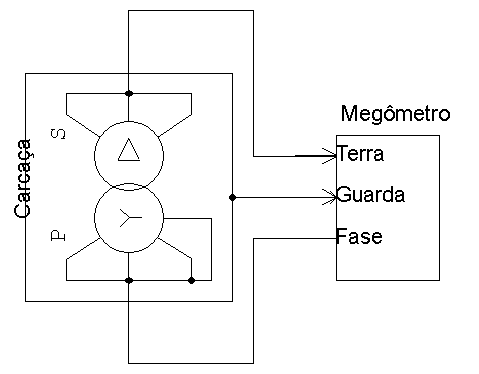
\includegraphics[scale=0.7]{./pic/EsquemaMegometro.png}
        \caption{Terminais do lado primário curto circuitados, Terminais do lado secundário curto circuitados, Fase ligado no primário (lado de A.T), neutro no secundário (lado B.T)e terminal de guarda ligada à carcaça do transformador}
\ContinuedFloat
\centering
\subfloat[Transformador 1]{
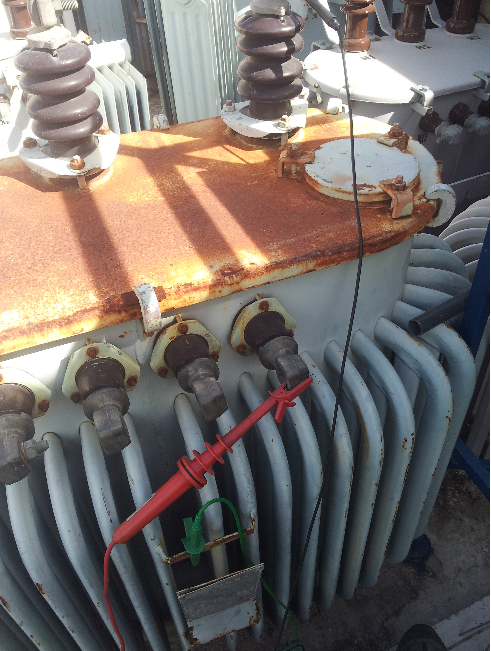
\includegraphics[width=6cm,height=6cm]{./pic/t1s.png}}
\subfloat[Transformador 2]{
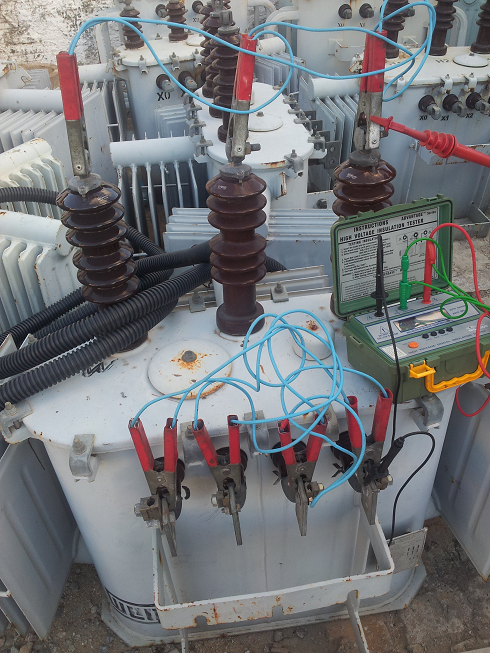
\includegraphics[width=6cm,height=6cm]{./pic/t2s.png}}
\qquad
\subfloat[Transformador 3]{
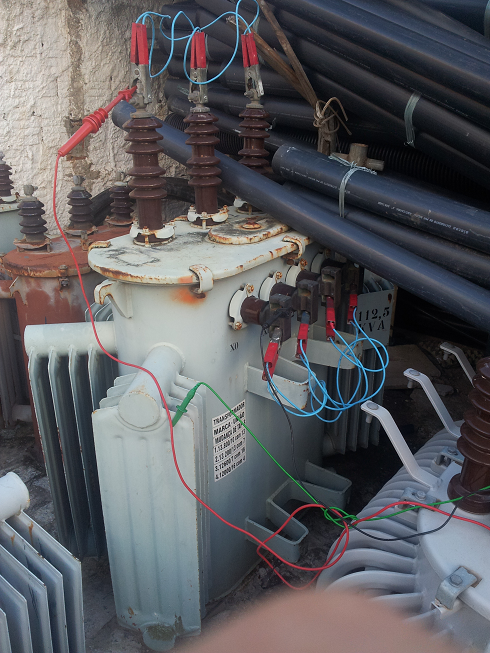
\includegraphics[width=6cm,height=6cm]{./pic/t3s.png}}
\subfloat[Transformador 4]{
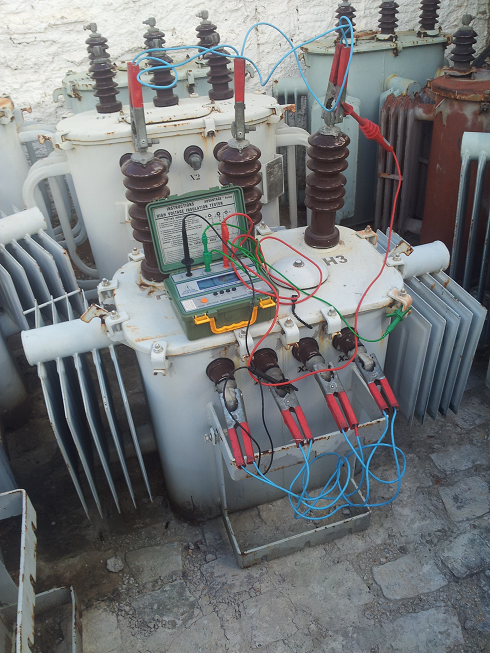
\includegraphics[width=6cm,height=6cm]{./pic/t4s.png}}
\end{figure}
\pagebreak

\begin{figure}
\centering
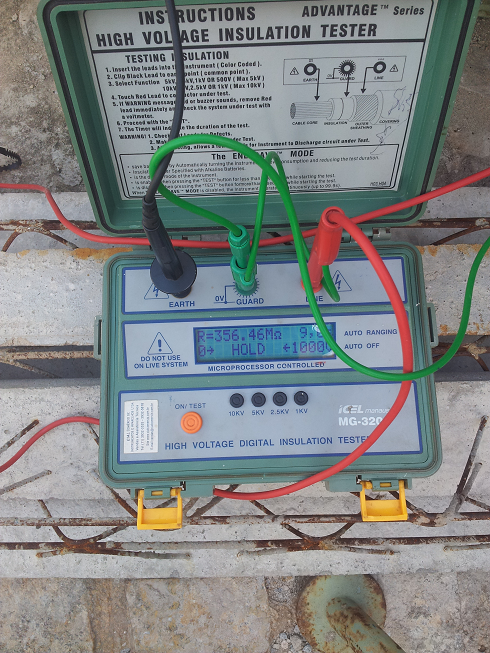
\includegraphics[width=6cm,height=6cm]{./pic/ExMe}
\caption[]{Megômetro MG-3200 da ICEL durante uma das medições}
\label{fig:ExMedição}
\end{figure}

\begin{table}[htbp]
  \centering

    \begin{tabular}{cccc}
    \toprule
    \textbf{Trafo} & \textbf{M1, Março, 14:00} & \textbf{M2, Março, 15:00} & \textbf{M3, Março, 16:00}\\
    \midrule
    1     & $419.05M\Omega$ &  $412.20M\Omega$ & $408.02M\Omega$ \\
    2     & $356.46M\Omega$ &  $368.71M\Omega$   & $371.95M\Omega$  \\
    3     & $54.64M\Omega$ & $53.67M\Omega$   & $52.81M\Omega$  \\
    4     & $290.10M\Omega$& $289.11M\Omega$   & $291.64M\Omega$  \\  
    \bottomrule
    \end{tabular}%
  \caption{Medição da Resistência de Continuidade dos Trafos}
\end{table}


\begin{table}[htbp]
  \centering

    \begin{tabular}{cccc}
    \toprule
    \textbf{Trafo} & \textbf{M1, Maio, 15:00} & \textbf{M2, Maio, 15:30} & \textbf{M3, Maio, 16:00}\\
    \midrule
    1     & $418.02M\Omega$ & $416.1M\Omega$  & $407.89M\Omega$  \\ 
    2     & $354.14M\Omega$ & $356.66M\Omega$   & $355.51M\Omega$   \\
    3     & $69.27M\Omega$ & $60.30M\Omega$   & $57.31M\Omega$  \\  
    4     & $285.51M\Omega$ & $287.37M\Omega$   & $286.13M\Omega$  \\  
    \bottomrule
    \end{tabular}%
  \caption{Medição da Resistência de Continuidade dos Trafos}
\end{table}


\subsection{Análise dos Resultados}
\samepage
A partir dessas tabelas, é possível concluir que os transformadores 1, 2 e 4 não apresentaram uma evolução significante nos valores da continuidade medidos ao longo de 2 meses, mantendo-se praticamente constante. No entanto o transformador 3 apresentou uma grande variação,o que indica que as características físicas internas ao transformador se alteraram de alguma forma neste período, de forma que é recomendável a abertura da tampa para checagem do óleo e dos enrolamentos antes de qualquer tentativa de religar o equipamento à rede elétrica.
\\
   %fotos


\section{Montagem de um Quadro de Força}

O quadro de força que foi montado e está descrito no diagrama unifilar da figura abaixo (página 10), consiste em:
\begin{itemize}
\item 7 disjuntores BT trifásicos, corrente nominal $I_n$=1600A, Cap. Interrupção = 36kA
\item 5 disjuntores BT trifásicos, corrente nominal $I_n$=450A, Cap. Interrupção = 36kA
\item 1 disjuntor BT trifásico, corrente nominal $I_n$ = 350A, Cap. Interrupção = 36kA
\item 1 disjuntor BT trifásico, corrente nominal $I_n$ = 250A, Cap. Interrupção = 36kA
\item 1 chave tripolar, corrente nominal 1600A
\item aproximadamente 53.5 metros de barramentos chatos de cobre pintado de $2.1/2"$ por $3/8"$
\end{itemize} 
Destes itens, dois disjuntores de baixa tensão trifásicos de corrente nominal 1600A protegem os transformadores. Um disjuntor de 1600A é para a proteção geral das cargas não essenciais. Um disjuntor de 1600A para a proteção geral das cargas essenciais. Dois disjuntores, um de 1600A que fica normalmente aberto e outro normalmente fechado além da chave tripolar são destinados para manobras com carga envolvendo a Unidade de Supervisão de Corrente Alternada para a entrada do grupo gerador. Um disjuntor de 1600A serve para a proteção de uma carga não especificada como essencial ou não essencial. \\

Os barramentos de cobre pintados de dimensões $2.1/2"$ por $3/8"$ ou 60 por 10 milímetros, com dois barramentos por fase tem capacidade de condução total de 1290A/$Barra\times Fase$ dando uma capacidade total de condução de  2580A/$Fase$, que implica na atuação dos disjuntores para proteção do barramento. \\

Das 7 cargas essenciais representadas no diagrama, 3 são protegidas individualmente por disjuntores, com correntes nominais iguais a 450, 450 e 250A.\\

Das 12 cargas não essenciais, 4 são protegidas individualmente por disjuntores de 450, 450, 450 e 350A de corrente nominal.
\\

Quando é necessária a atuação do grupo gerador, os dois disjuntores no caminho normalmente fechado da alimentação das cargas essenciais são abertos, muda-se a posição da chave tripolar e fecha-se o disjuntor normalmente aberto, de forma que o grupo gerador alimenta a carga essencial sem que alimente ou interaja com a rede elétrica. 

\begin{figure}
\centering
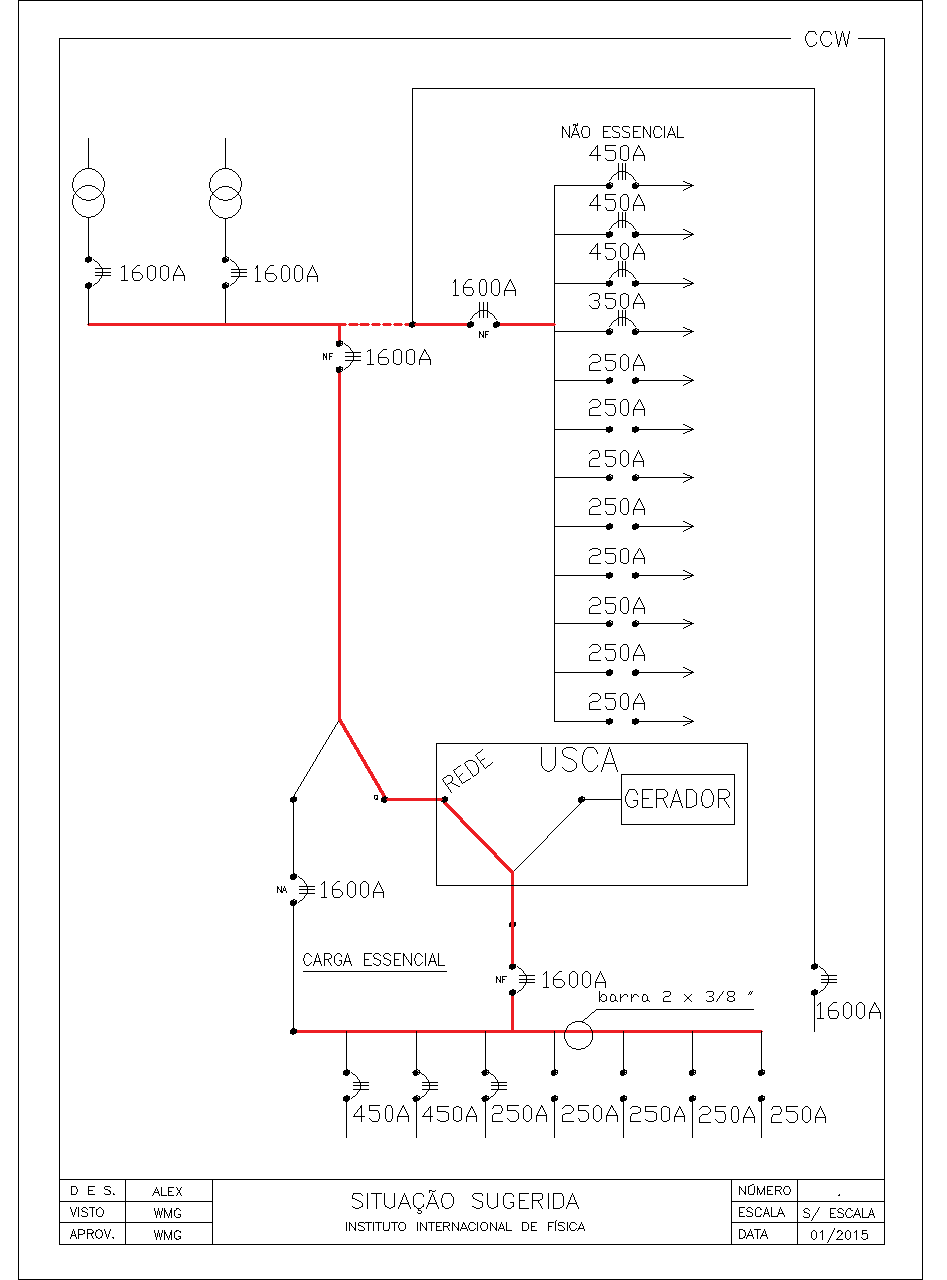
\includegraphics[width=12cm,height=15cm]{./pic/EsquemaQuadro.png}
\caption[]{Diagrama unifilar do Quadro de Força}
\label{fig:EsquemaQuadro}
\end{figure}


\begin{figure}
\ContinuedFloat
\centering
\subfloat[Disjuntores de Carga Essencial]{
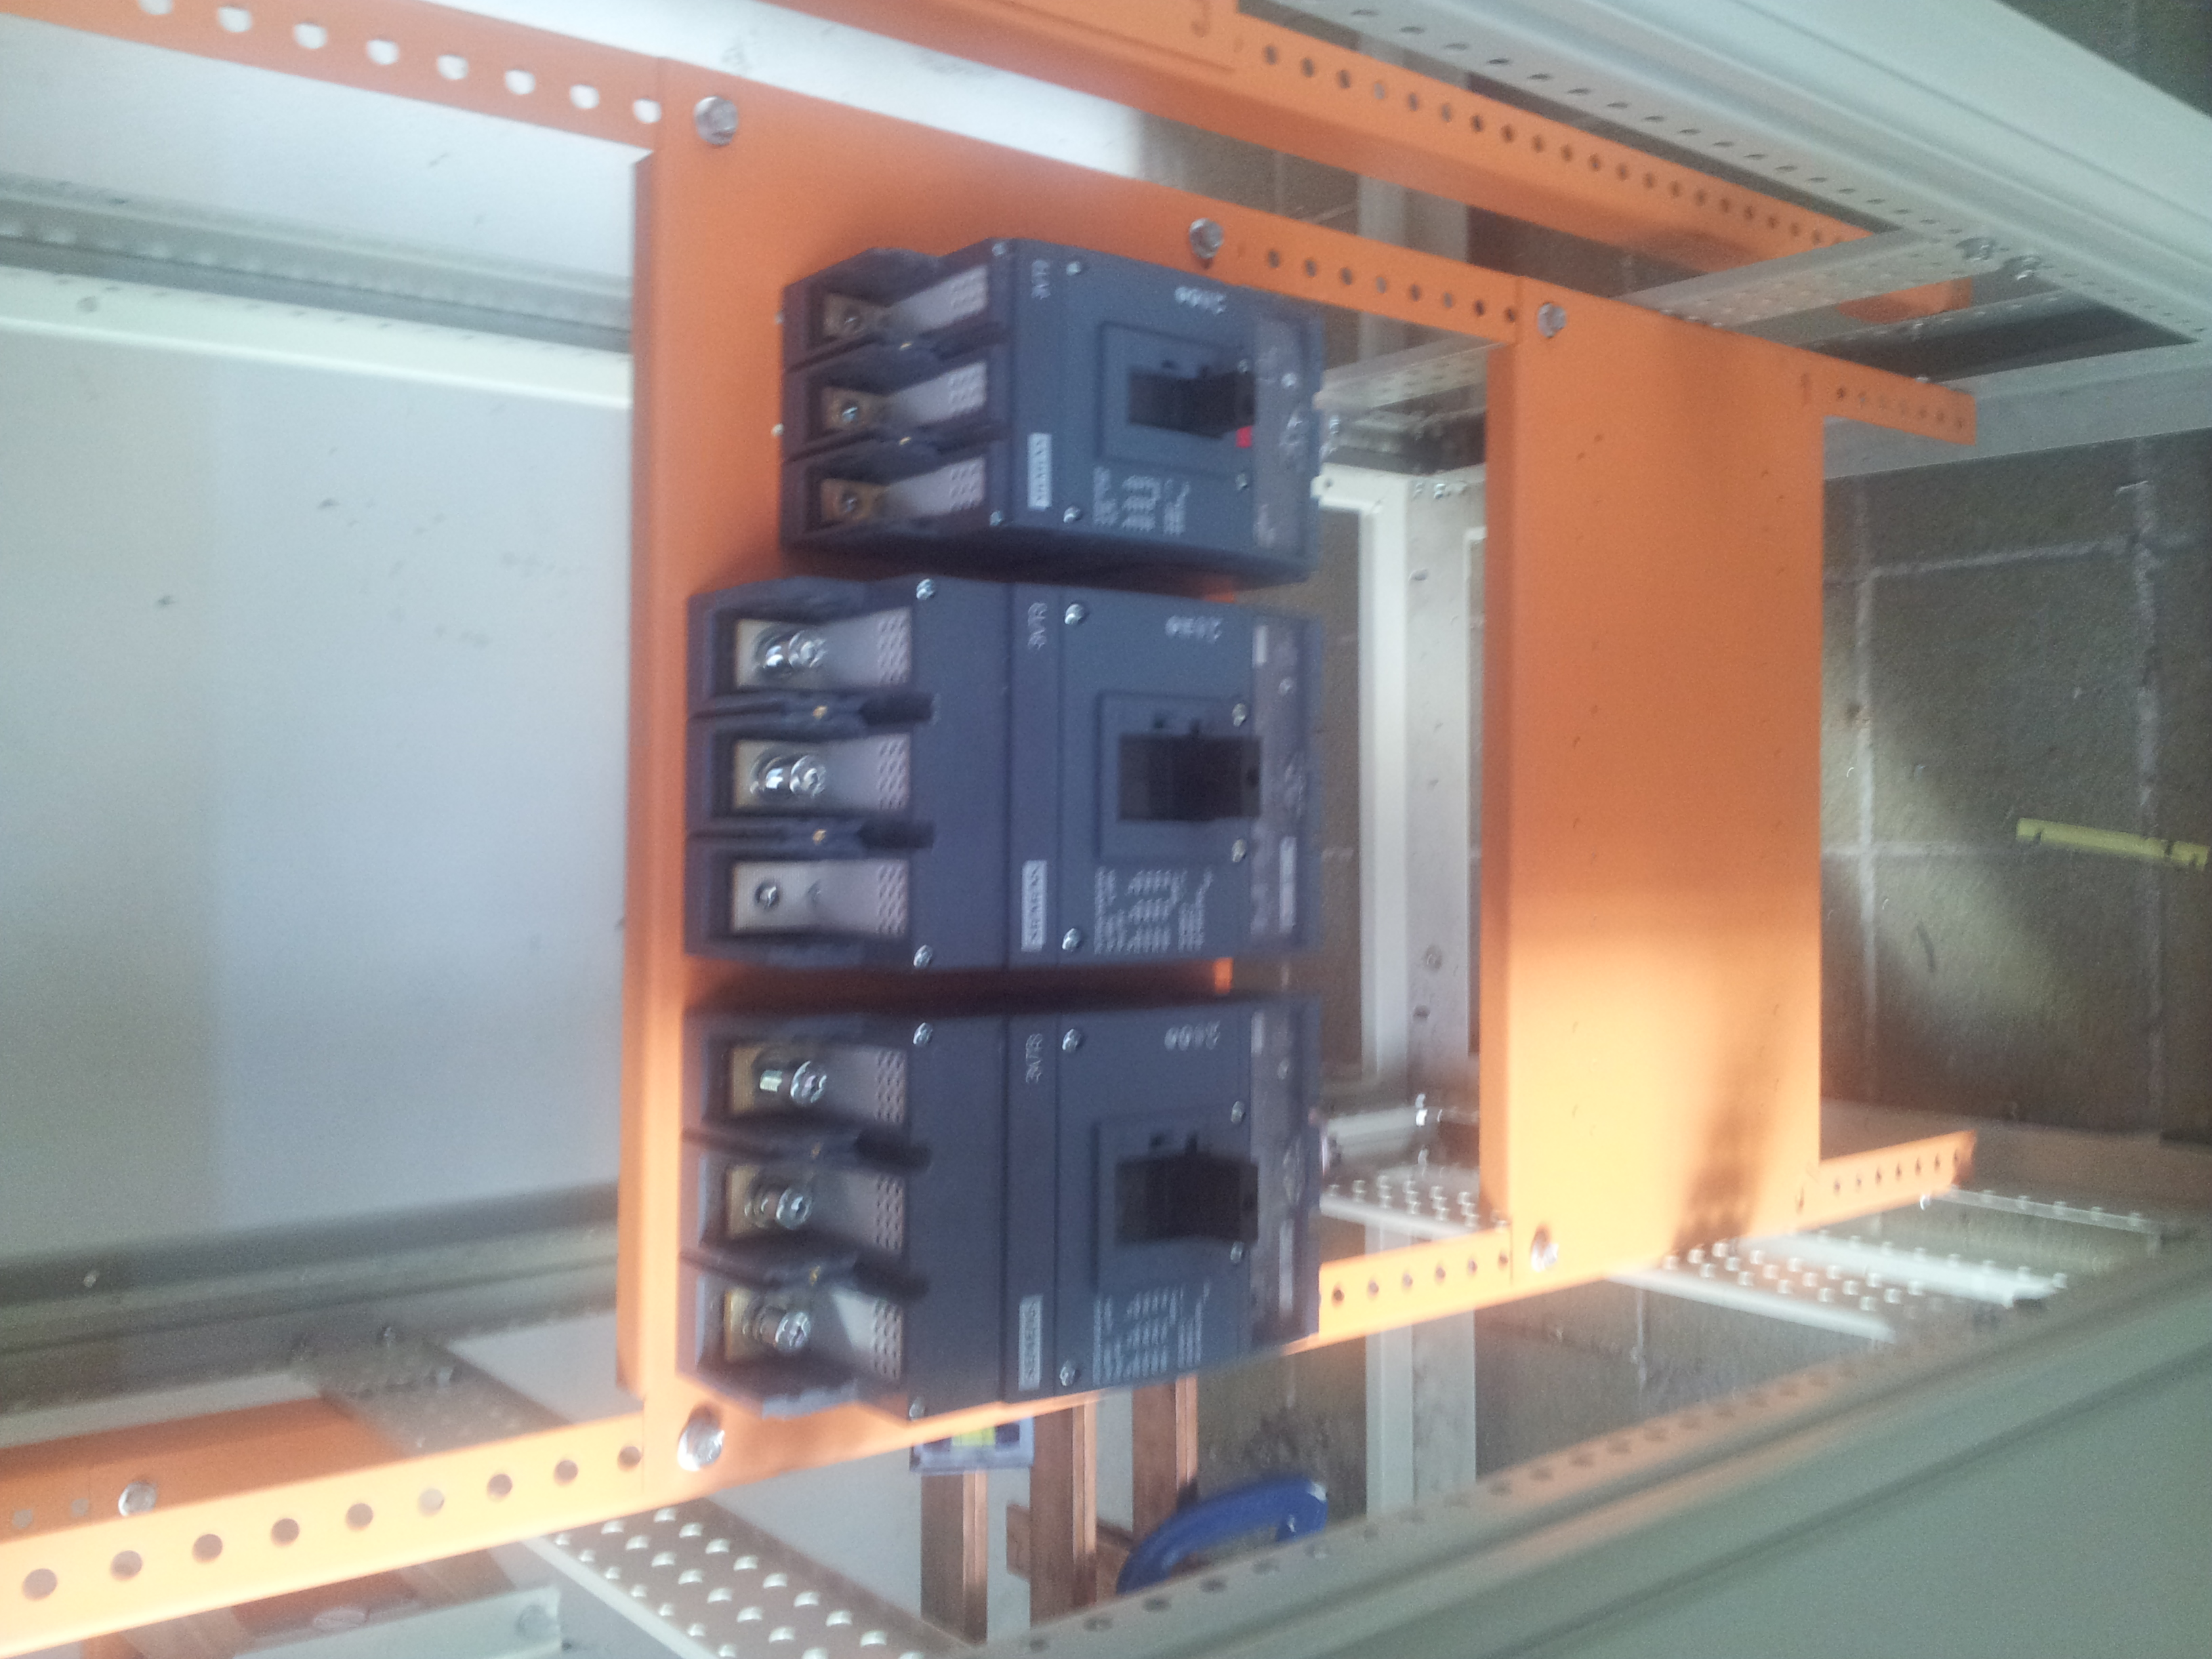
\includegraphics[width=5cm,height=6cm, angle =90]{./pic/q1.jpg}}
\subfloat[Barramentos (Azul, Branco, Roxo)]{
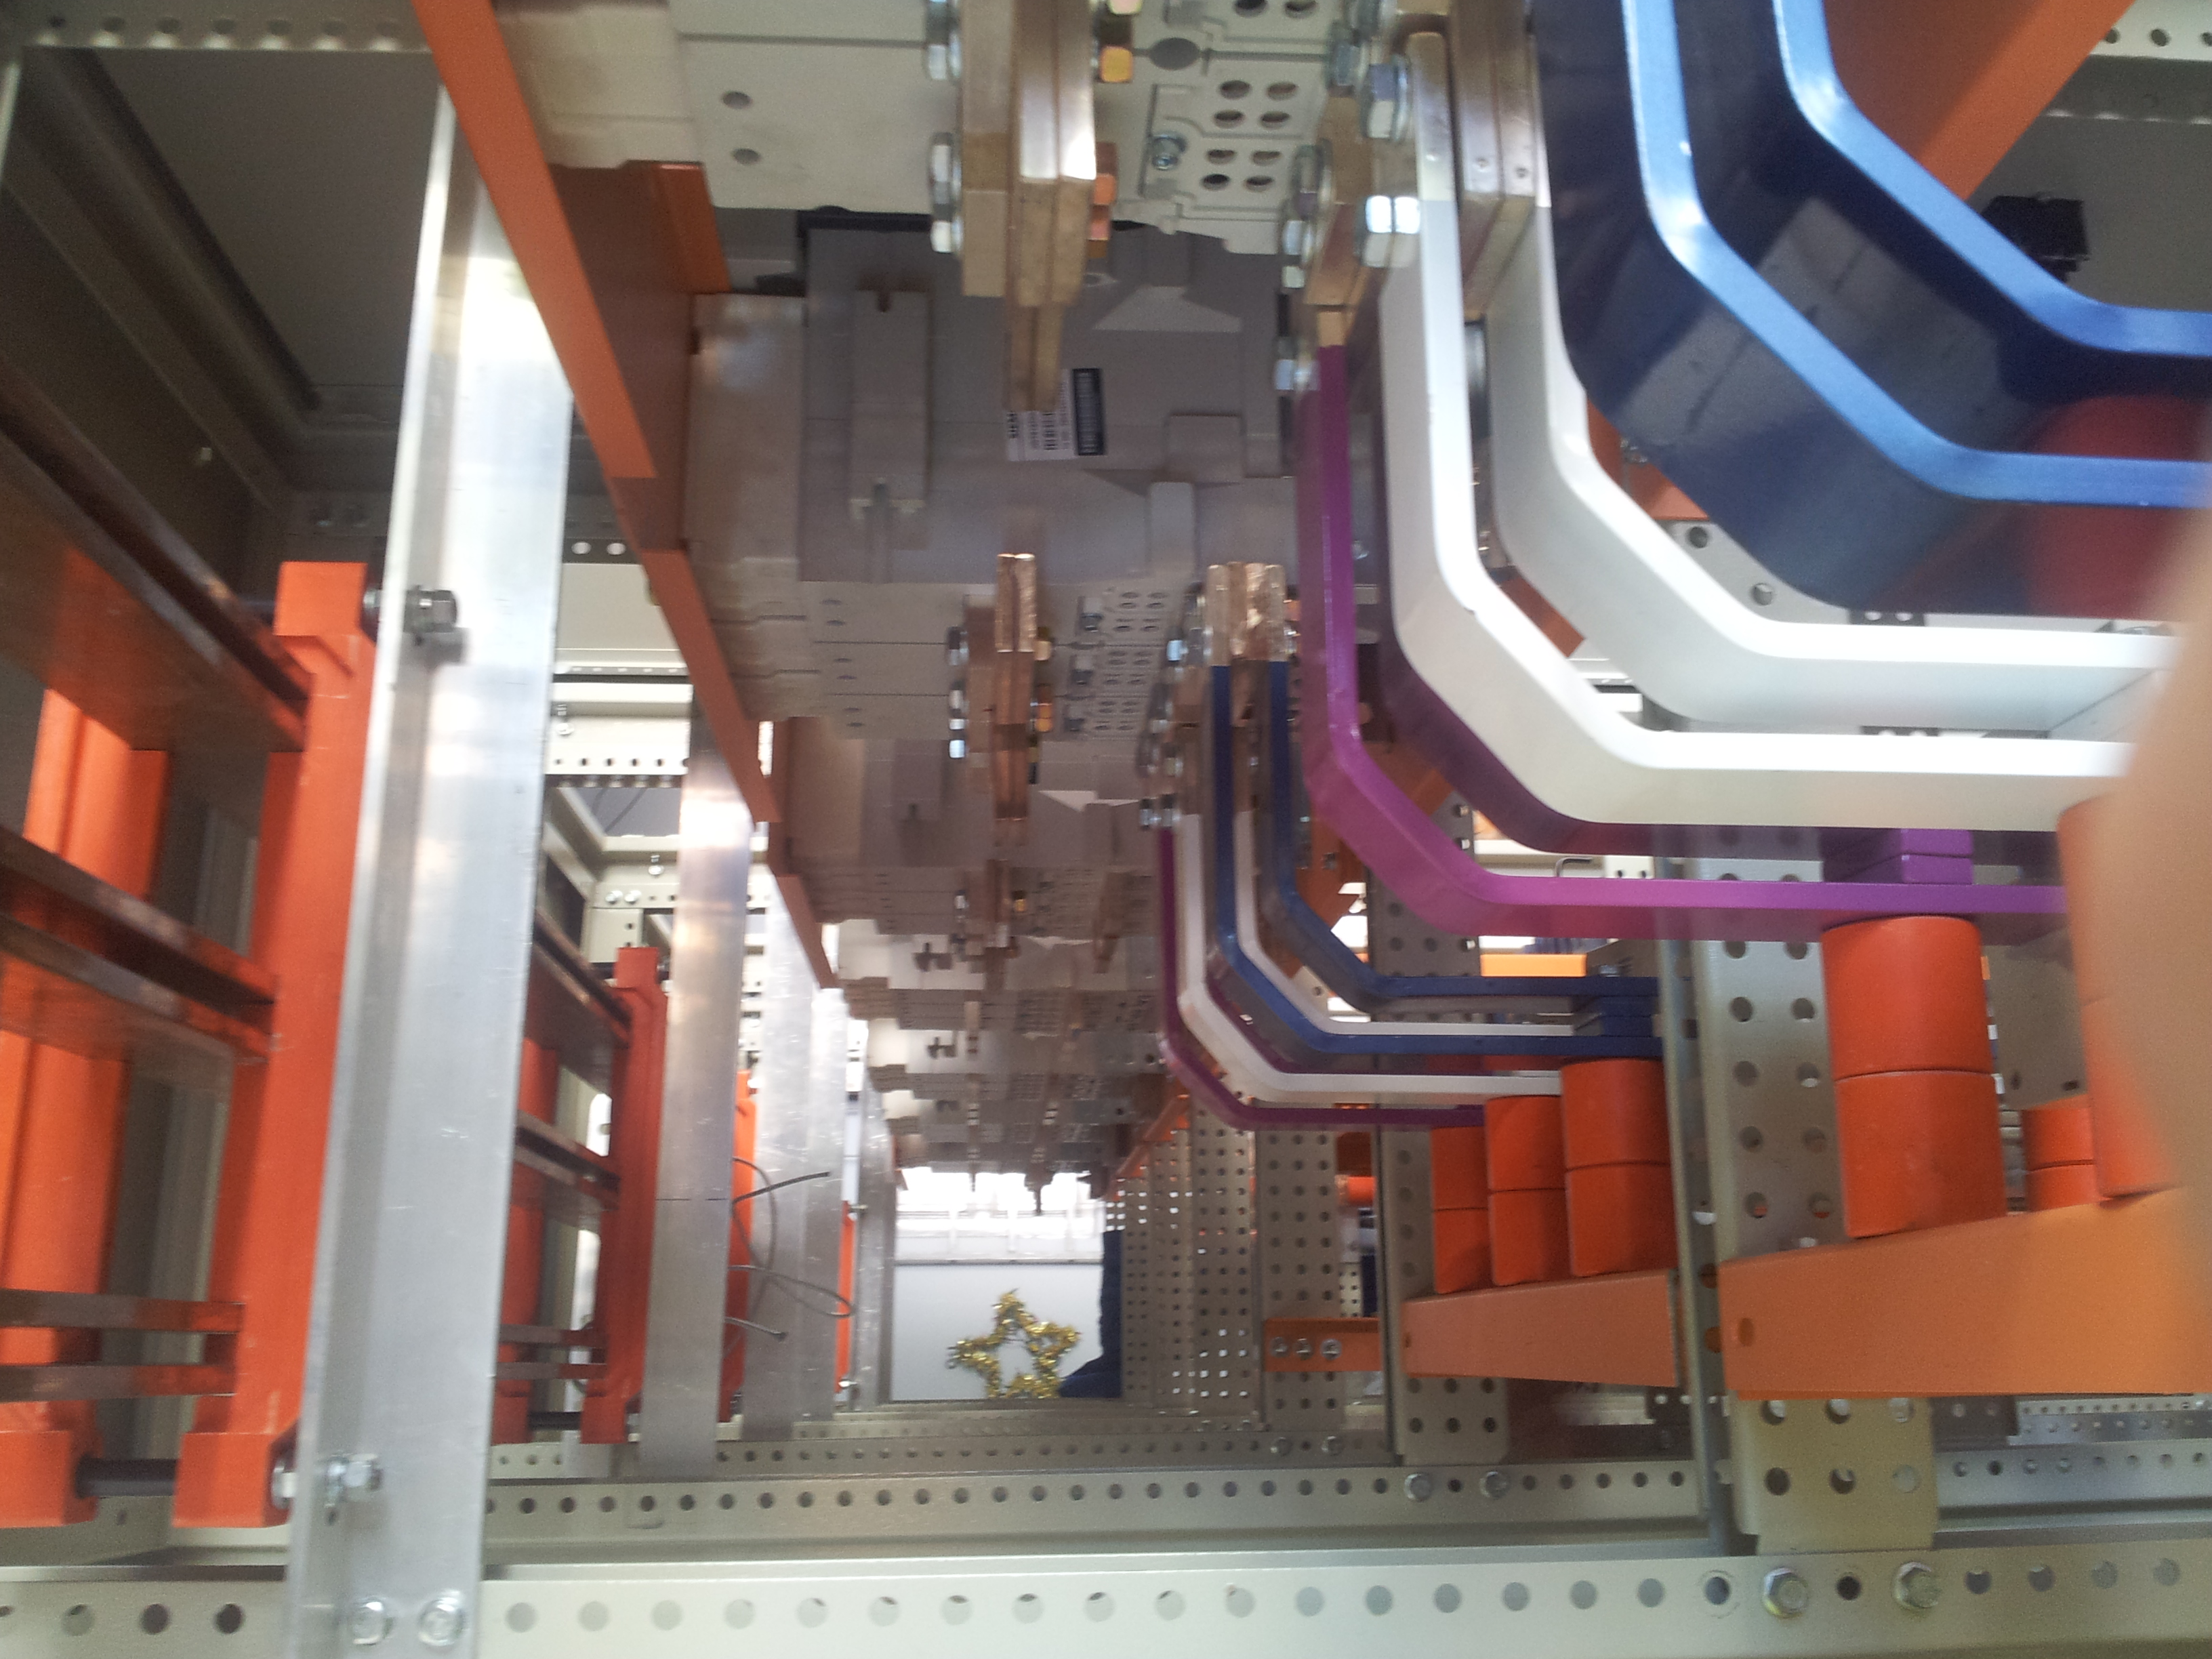
\includegraphics[width=5cm,height=6cm]{./pic/q2.jpg}}
\subfloat[TCs]{
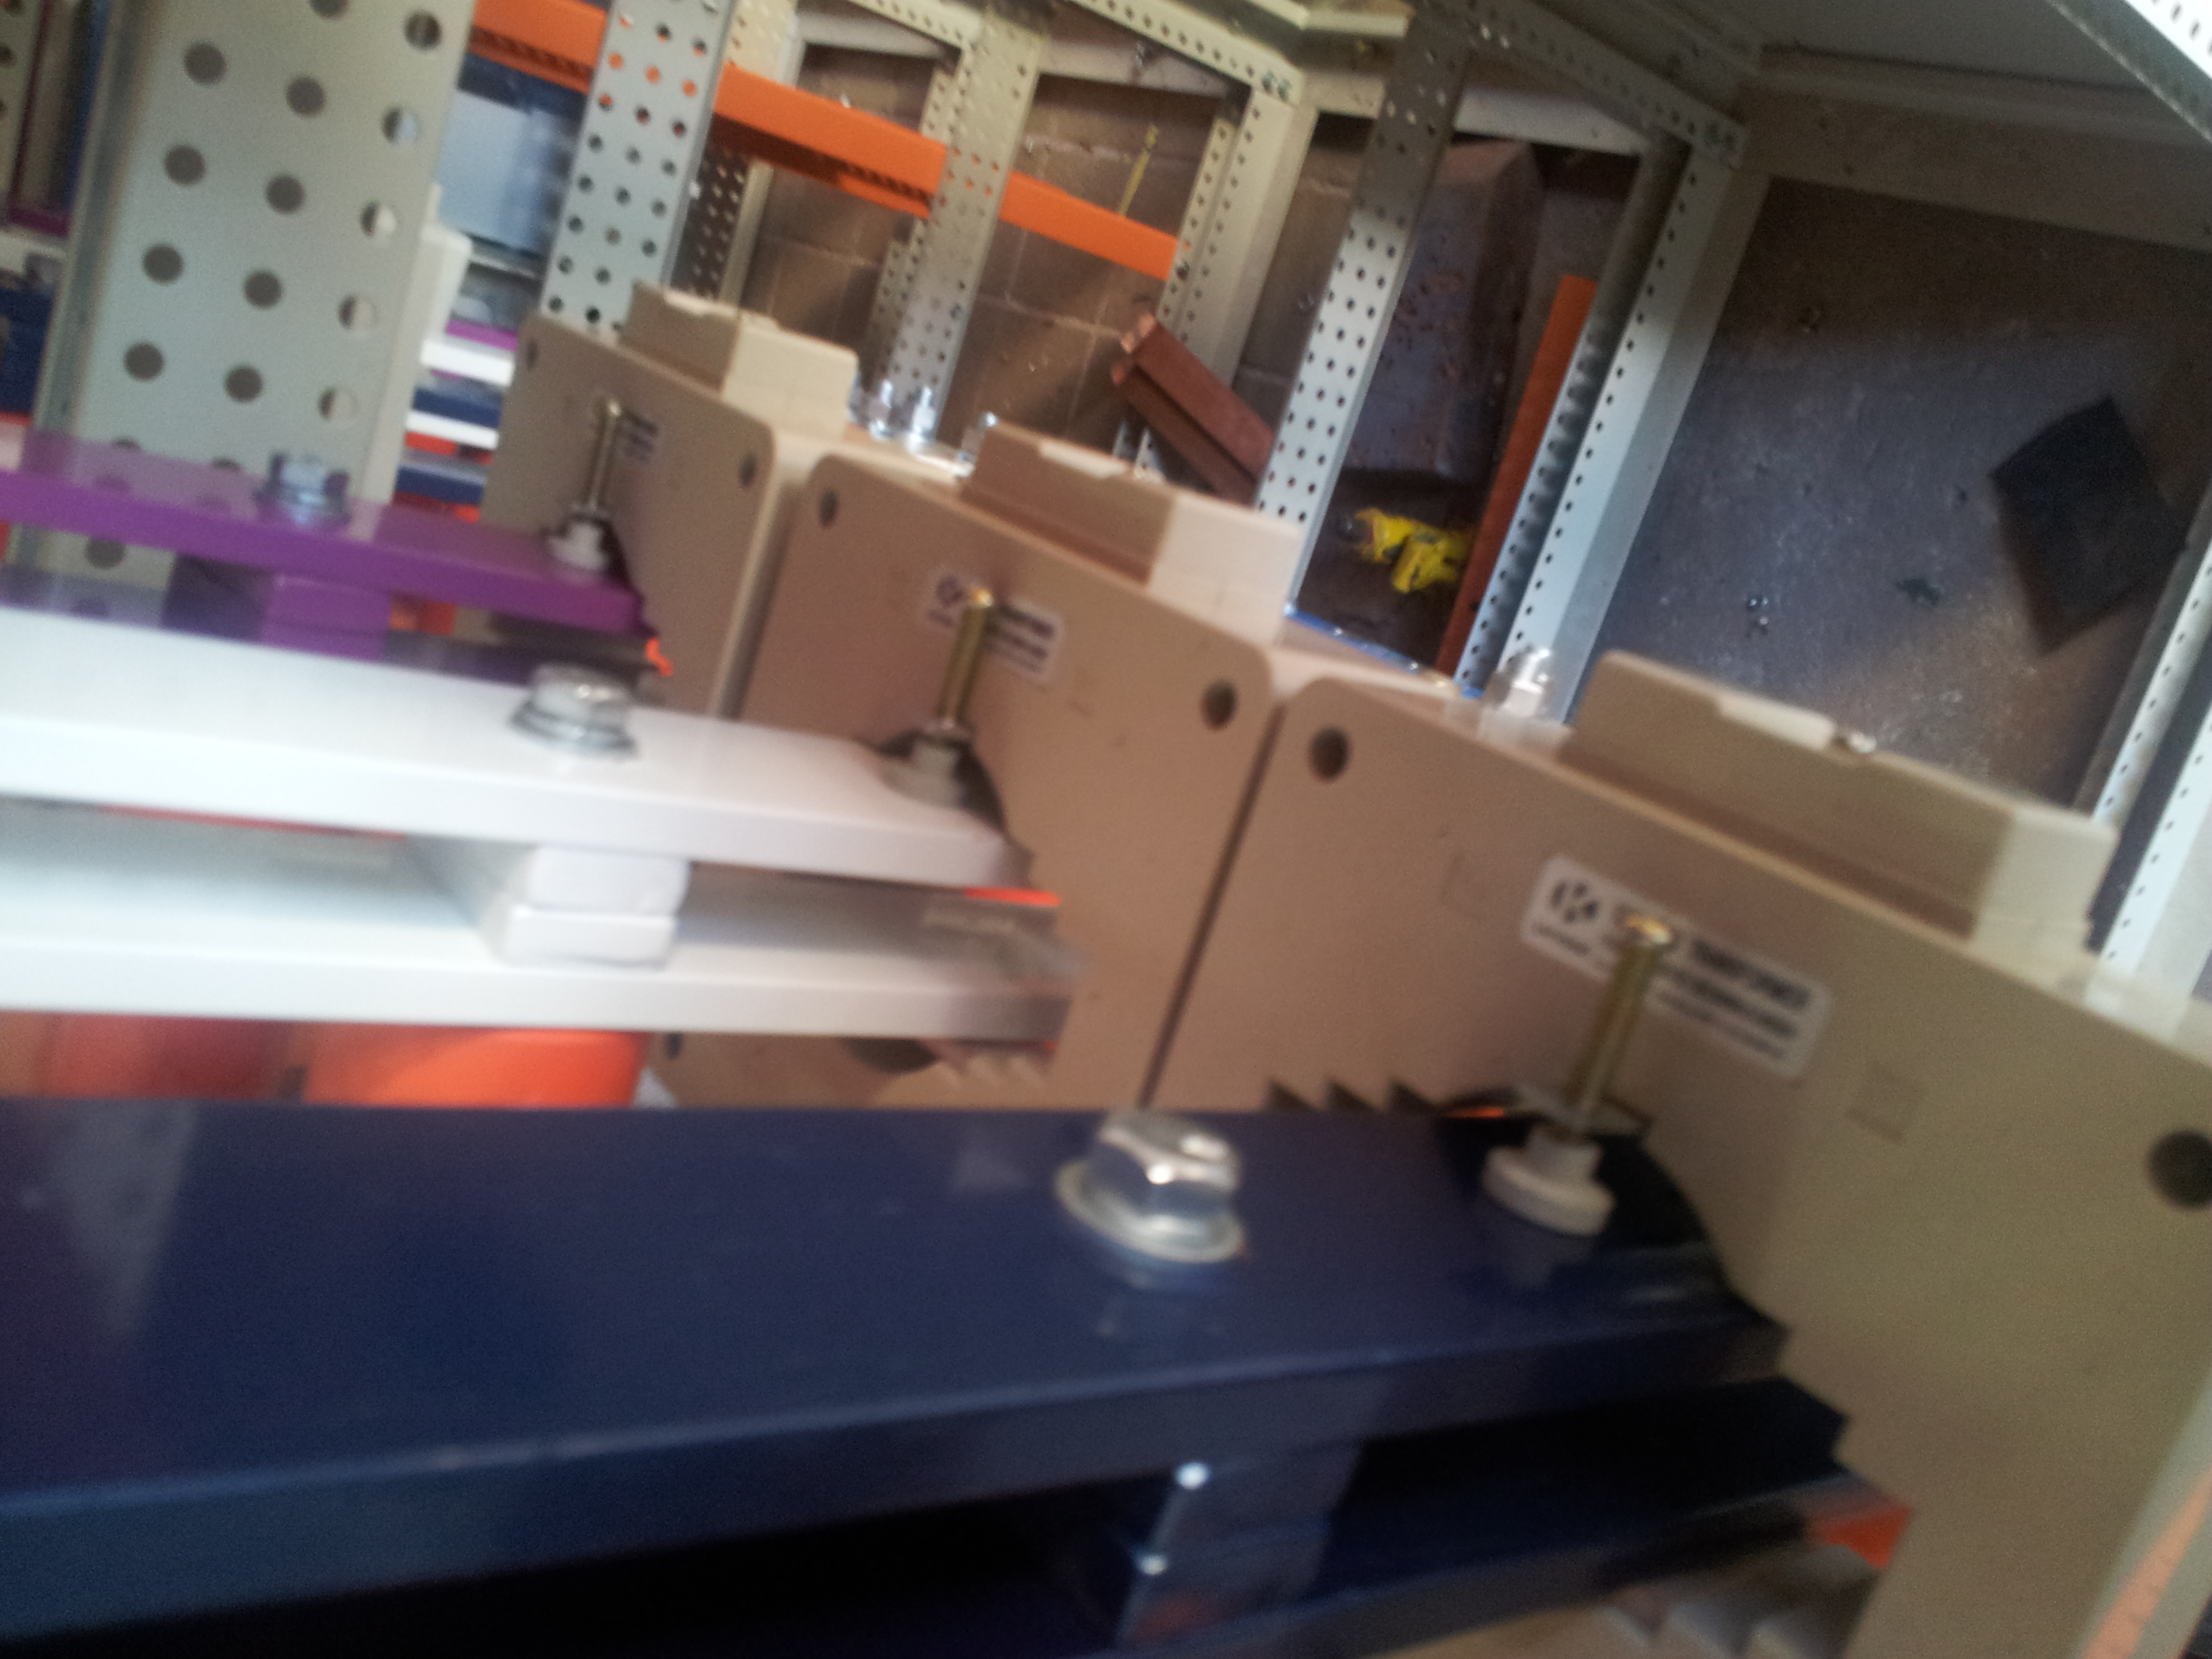
\includegraphics[width=5cm,height=6cm]{./pic/q3.jpg}}
\qquad
\subfloat[Disjuntores de Carga Não Essencial]{
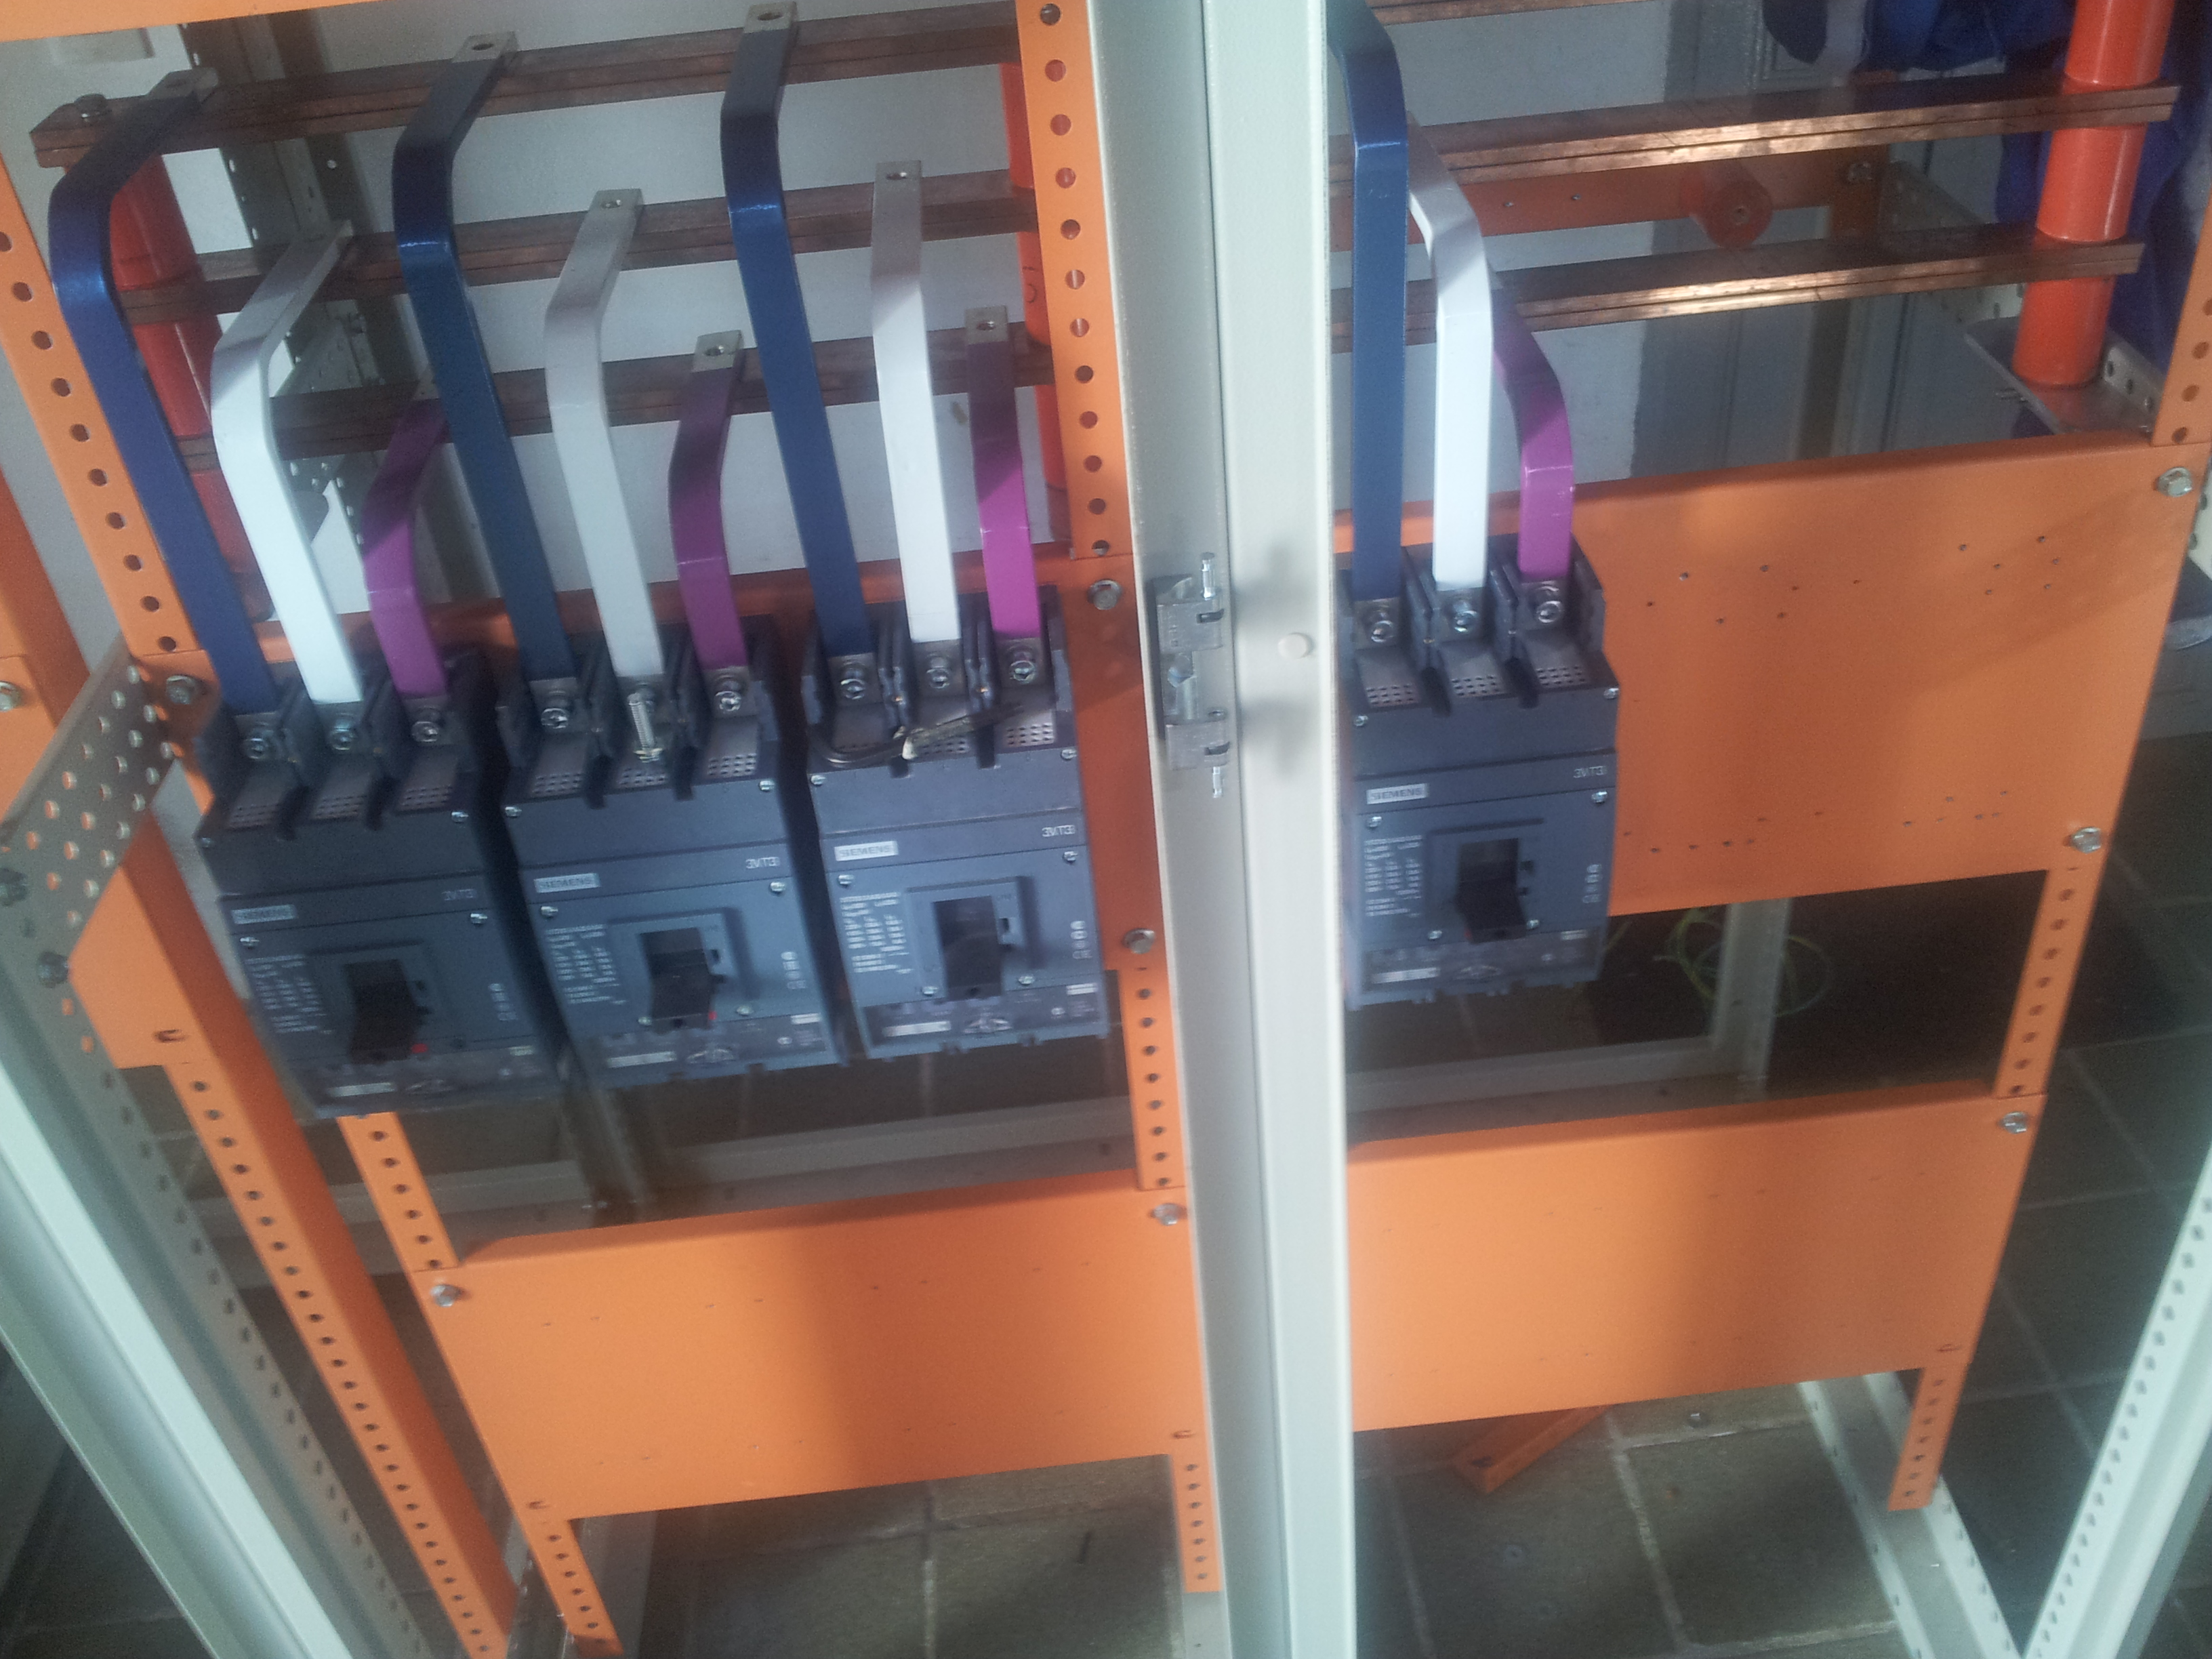
\includegraphics[width=6cm,height=6cm]{./pic/q4.jpg}}
\subfloat[Disjuntores e Medidores dos Trafos e Chave Tripolar]{
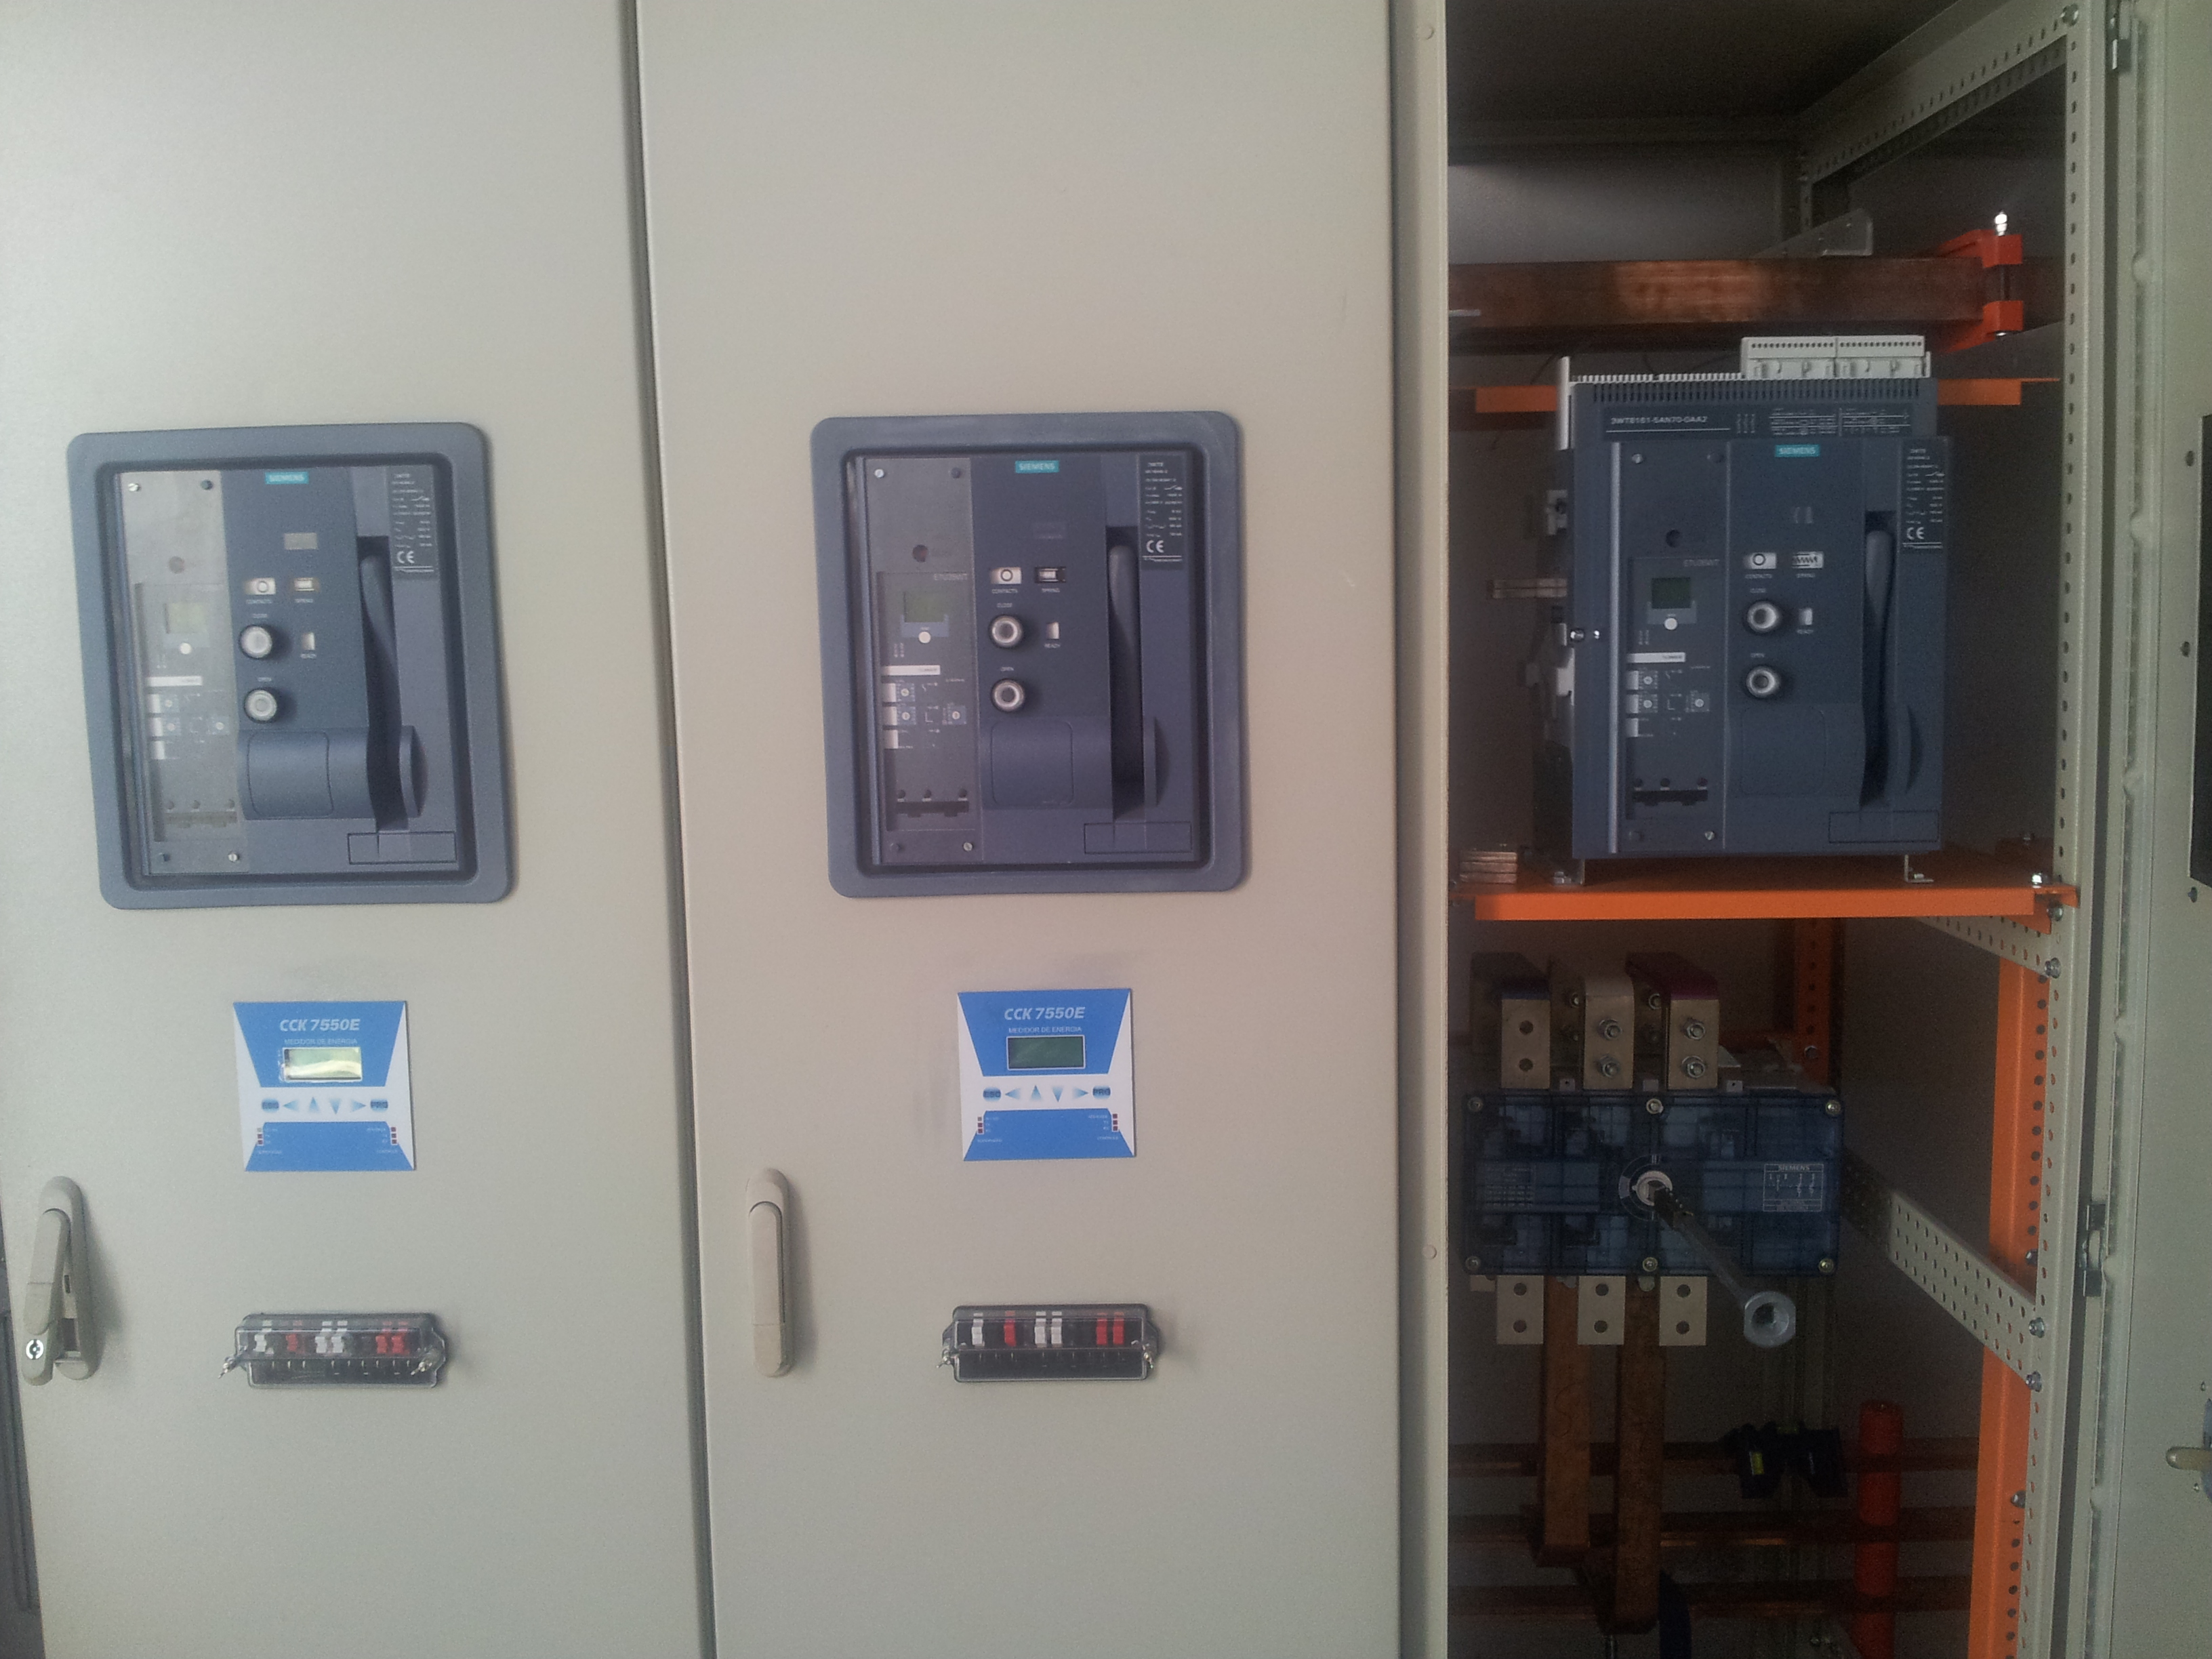
\includegraphics[width=6cm,height=6cm]{./pic/q5.jpg}}
\end{figure}
\pagebreak

%cabo de cobre nu 336,4 AWG CAA (170$mm^2$ de secção transversal com alma de aço)
\begin{figure}
\centering
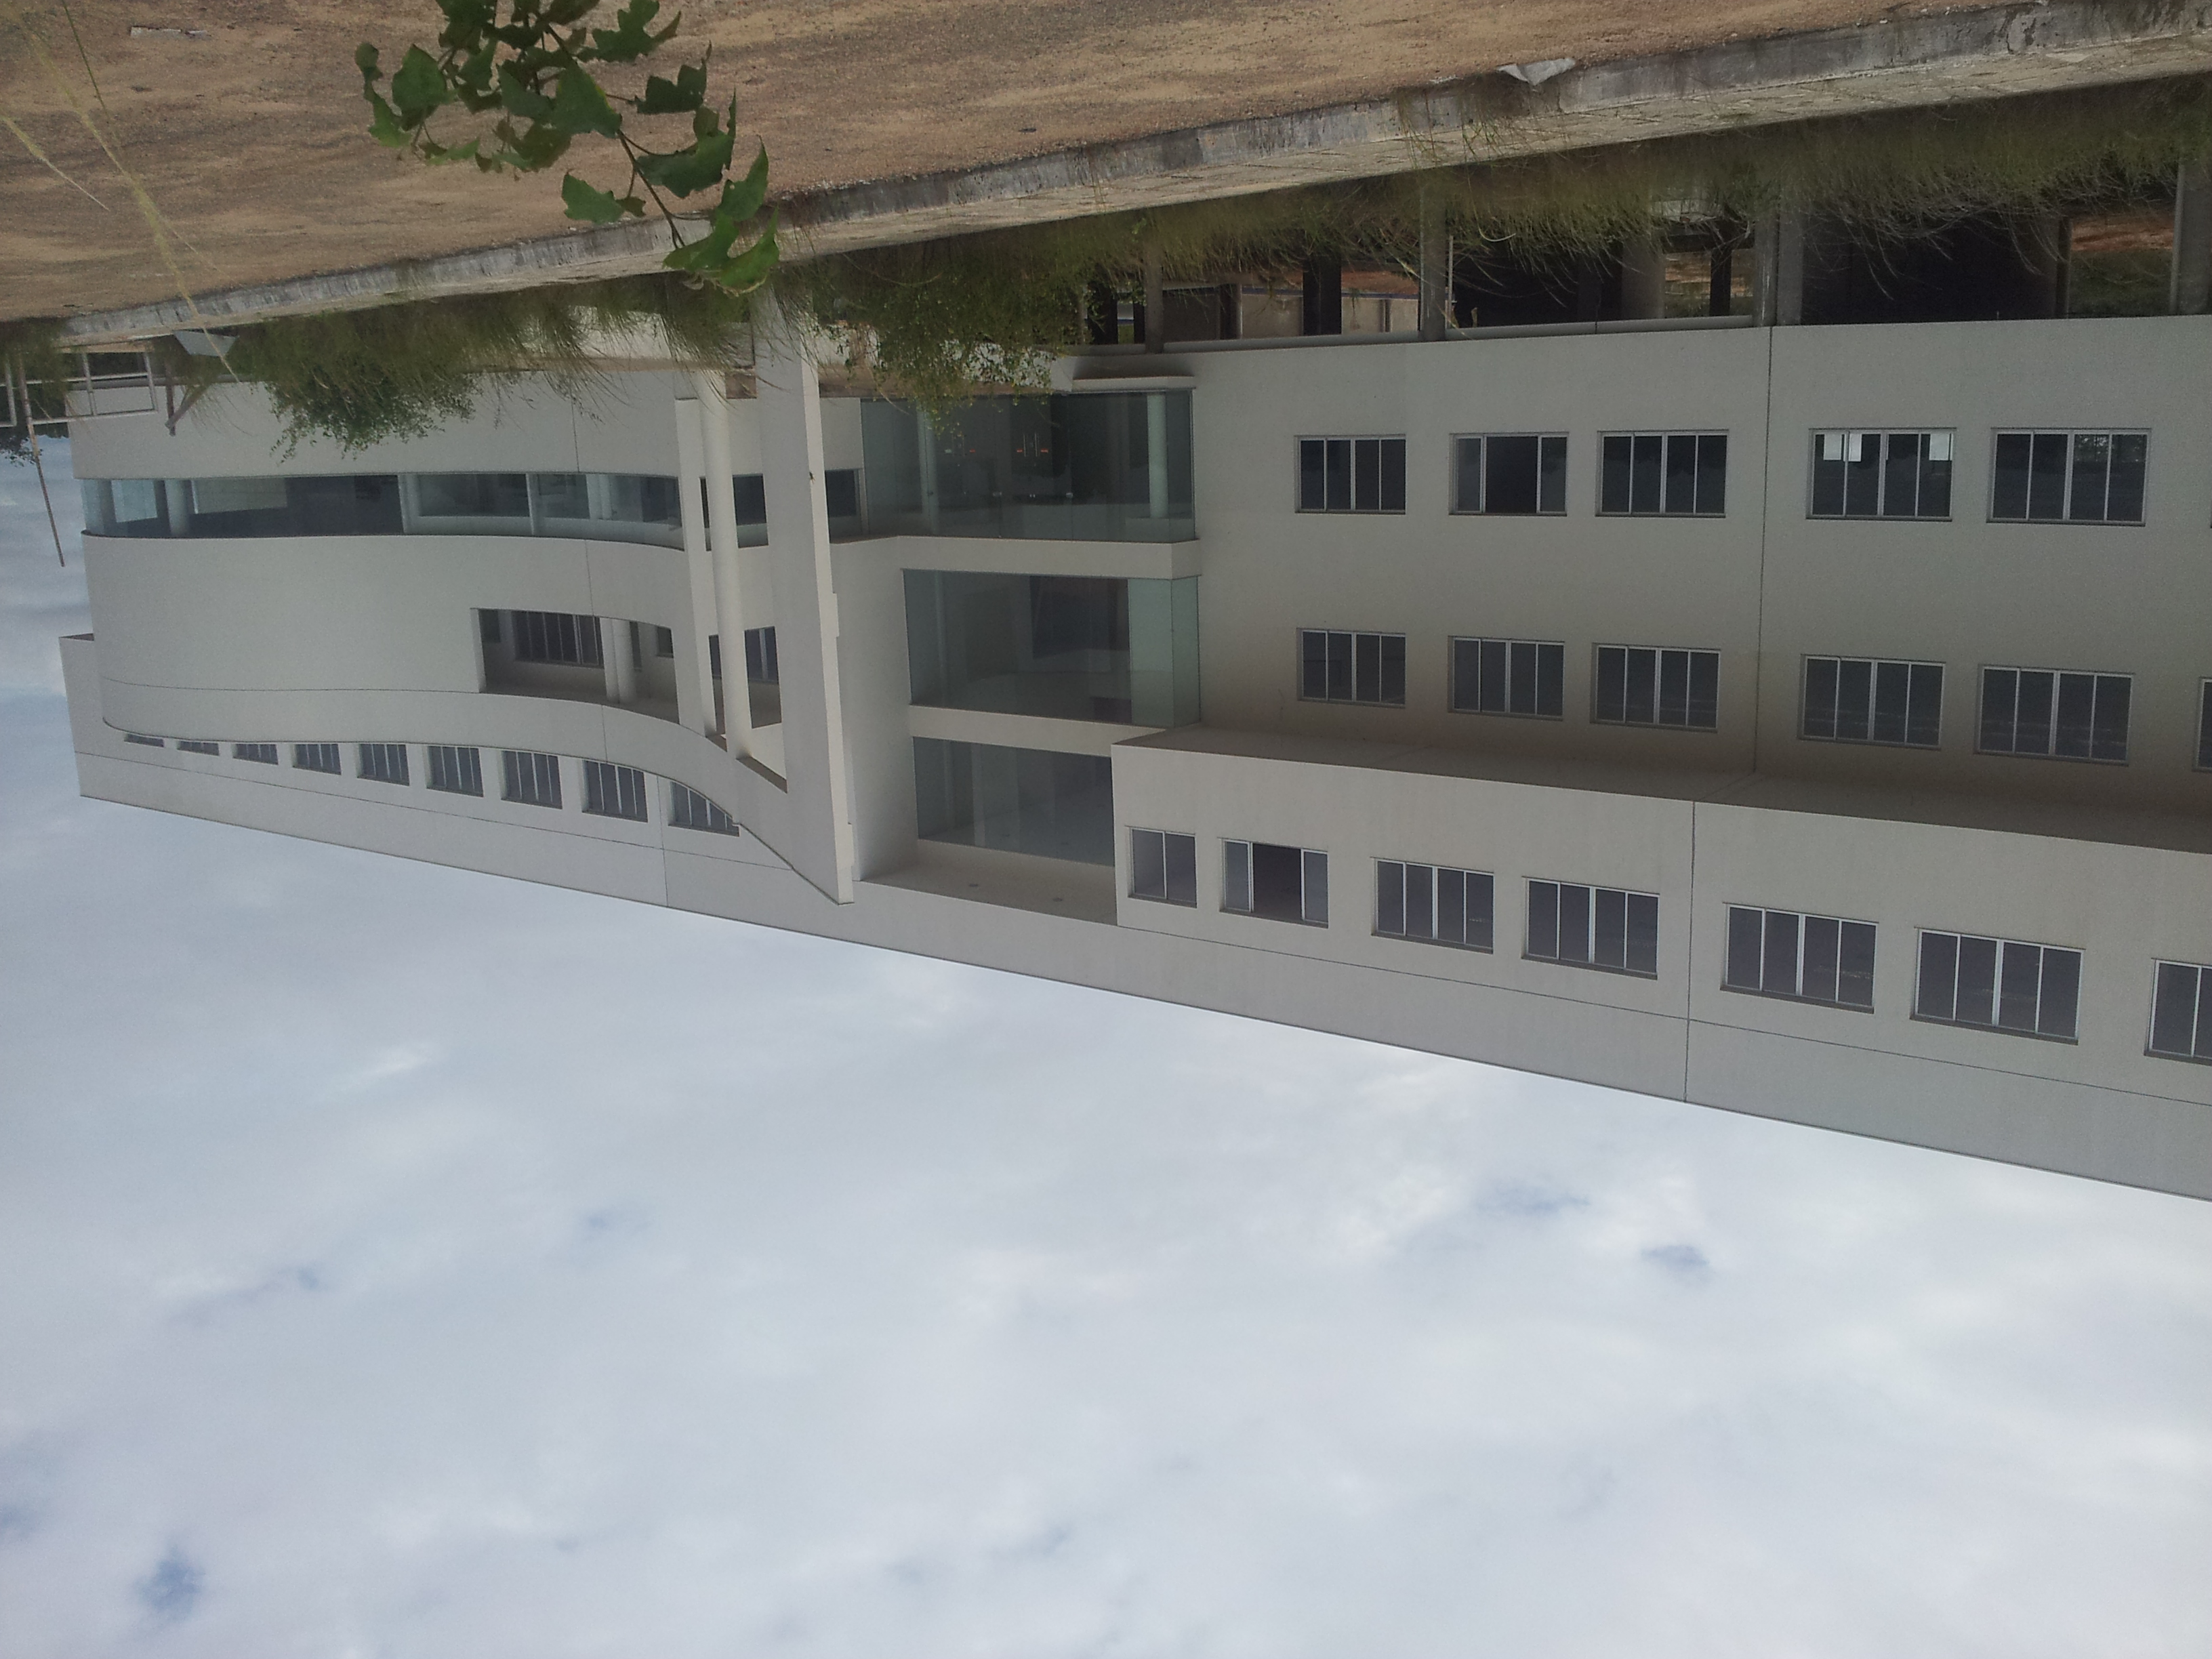
\includegraphics[width=15cm,height=10cm, angle=180]{./pic/PredioInstituto.jpg}
\caption{Futuros laboratórios do Campus do Cérebro em Macaíba}
\label{fig:PredioInstituto}
\end{figure}
\section{Acompanhamento da Obra do Campus da UFRN em Macaíba}
Foi possível acompanhar a obra e aprender sobre o padrão de estruturas para a rede de média tensão 13.8kV e sobre os materiais e equipamentos usados, pude ver como se dá a colocação de luminárias em poste tubular com a ajuda de um munck montado em caminhão.\\



\subsection{Projeto da Rede Elétrica do Campus do Cérebro}
O projeto da rede elétrica tem dimensões bastante extensas em se tratando de um campus. Como este relatório não é capaz de conter as minúcias do projeto escolhi anexá-lo digitalmente.\\

\begin{figure}
\centering
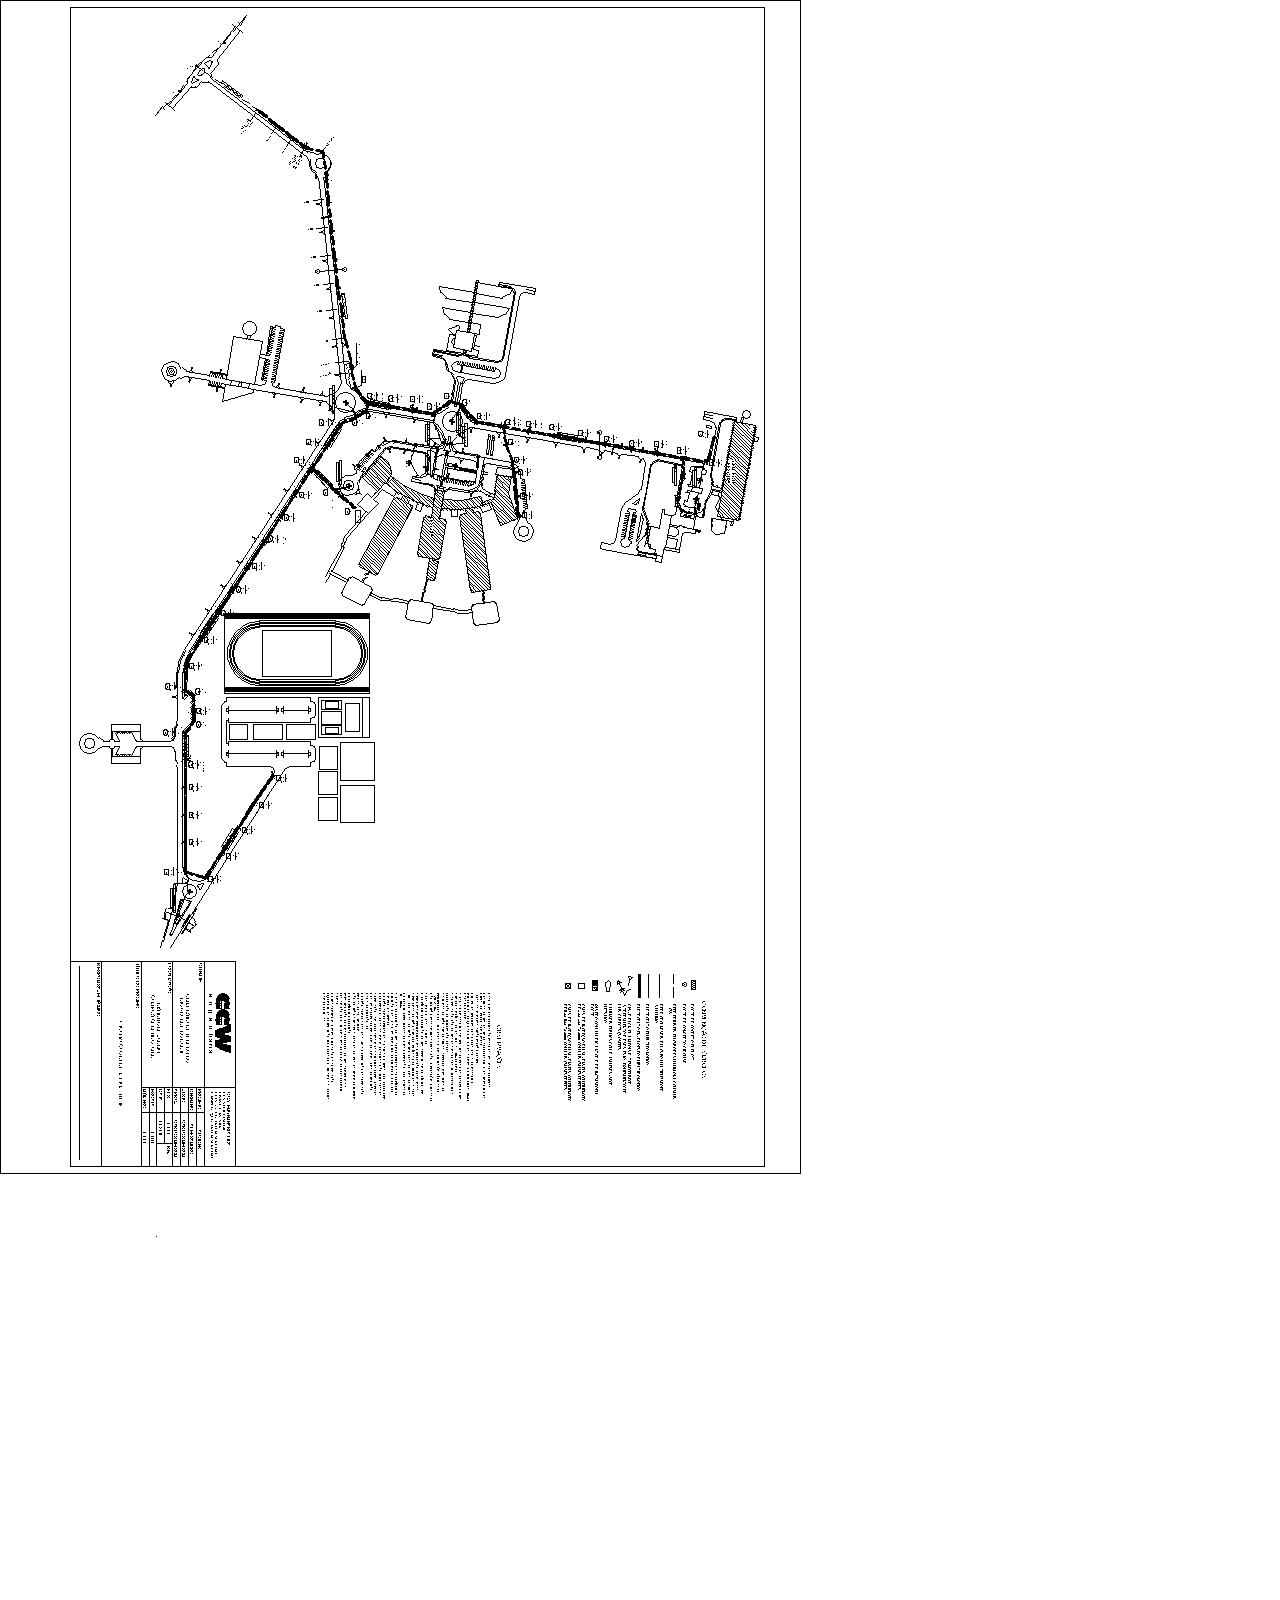
\includegraphics[width=12cm,height=16cm, angle = 90]{./pic/ATREDE.jpg}
\caption{Vista com zoom mínimo do projeto: No canto inferior esquerdo está o ponto de entrega de energia da concessionária que vai até um ponto central onde há uma cabine de medição e proteção primária que alimenta o prédio na parte superior do desenho. No canto inferior direito se encontra a entrada física do campus}
\label{fig:Projeto}
\end{figure}
\begin{figure}
\centering
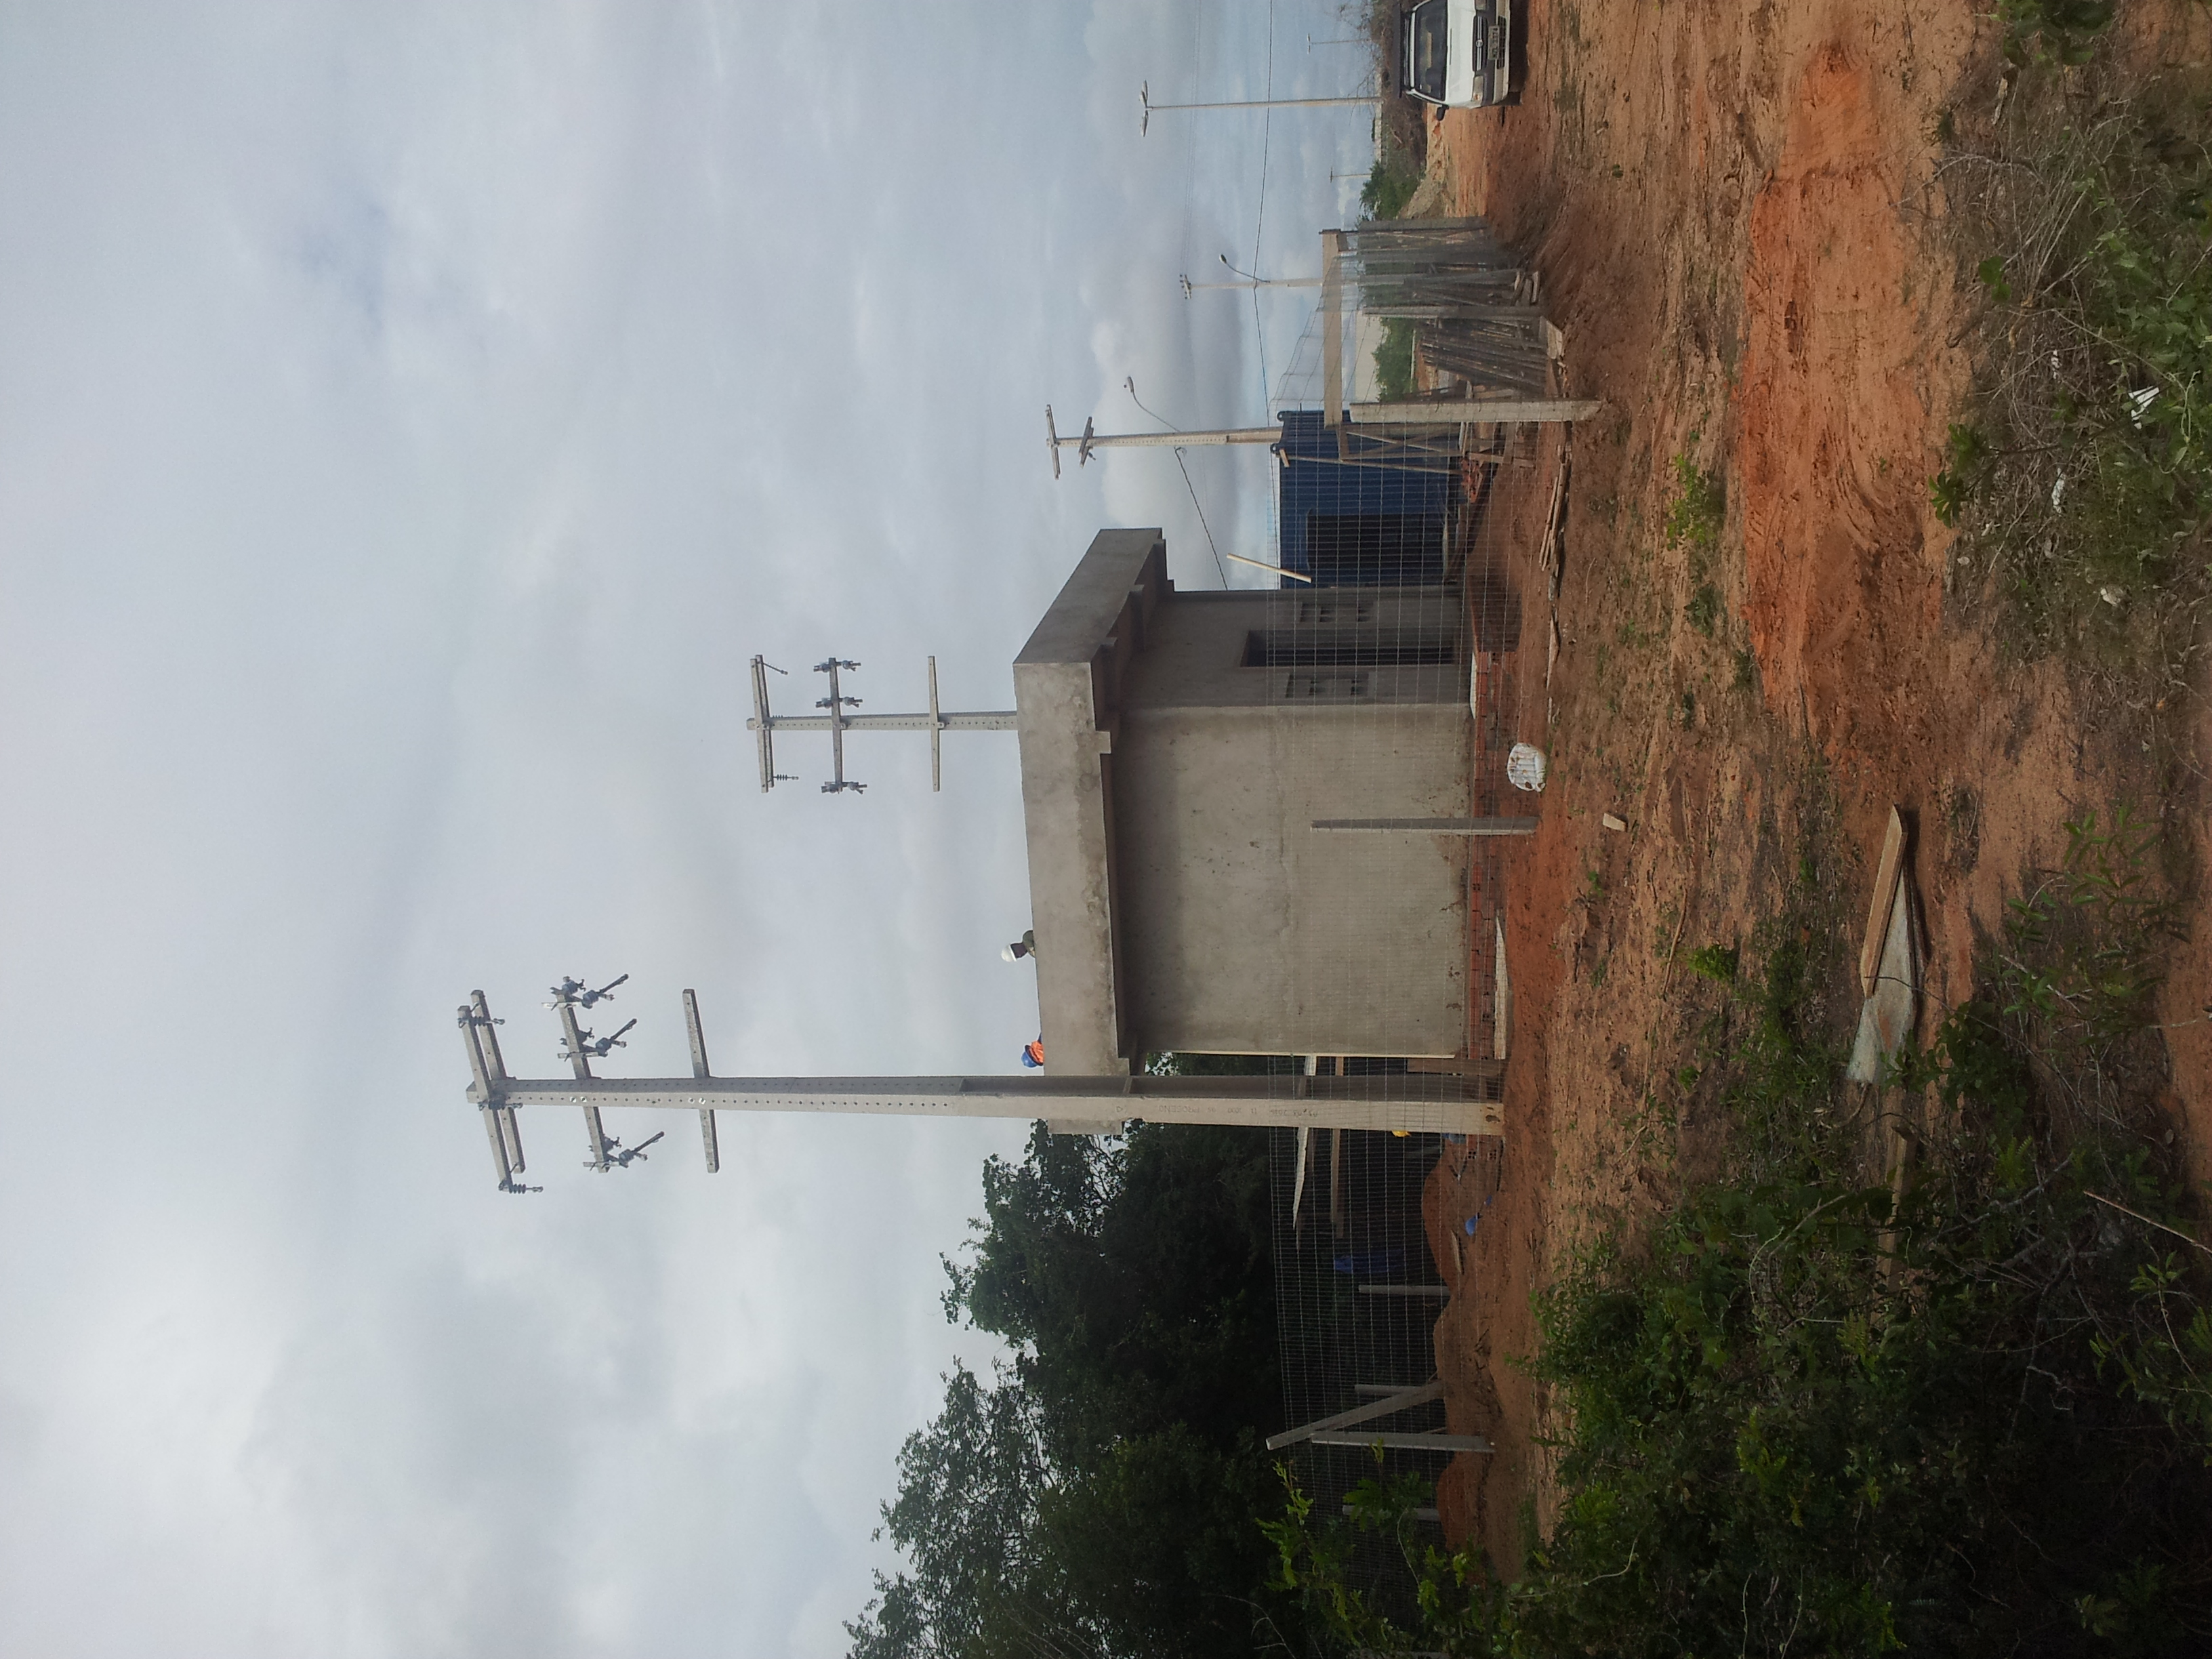
\includegraphics[width=7cm,height=10cm, angle = 270]{./pic/Cabine_P.jpg}
\caption{Cabine de Medição e Proteção}
\label{fig:Cabine}
\end{figure}
\subsection{Padrão de Estruturas}
Me familiarizei com os diversos padrões de estruturas de sustentação para a rede de média tensão, onde as estruturas do tipo N1 conduzem o cabo em linha reta com angulações menores que $6^\circ$, estruturas do tipo N2 conduzem o cabo com angulações de até $30^\circ$ e estruturas do tipo N3 servem para amarração da linha e para derivação em ângulos fechados onde o esforço que o poste deve ser capaz de suportar cresce quanto maiores forem as angulações que este deve suportar e quanto maior a massa dos cabos que devem ser sustentados. No caso desta obra a rede de média tensão foi feita inteiramente em cabo 336,4 AWG CAA que corresponde a um cabo com 170$mm^2$ de secção transversal com alma de aço. Podemos visualizar alguns exemplos nas figuras de letra "j", "k" e "l":\\

\begin{figure}
\ContinuedFloat
\centering
\subfloat[Estrutura N1-T (Trafo montado)]{
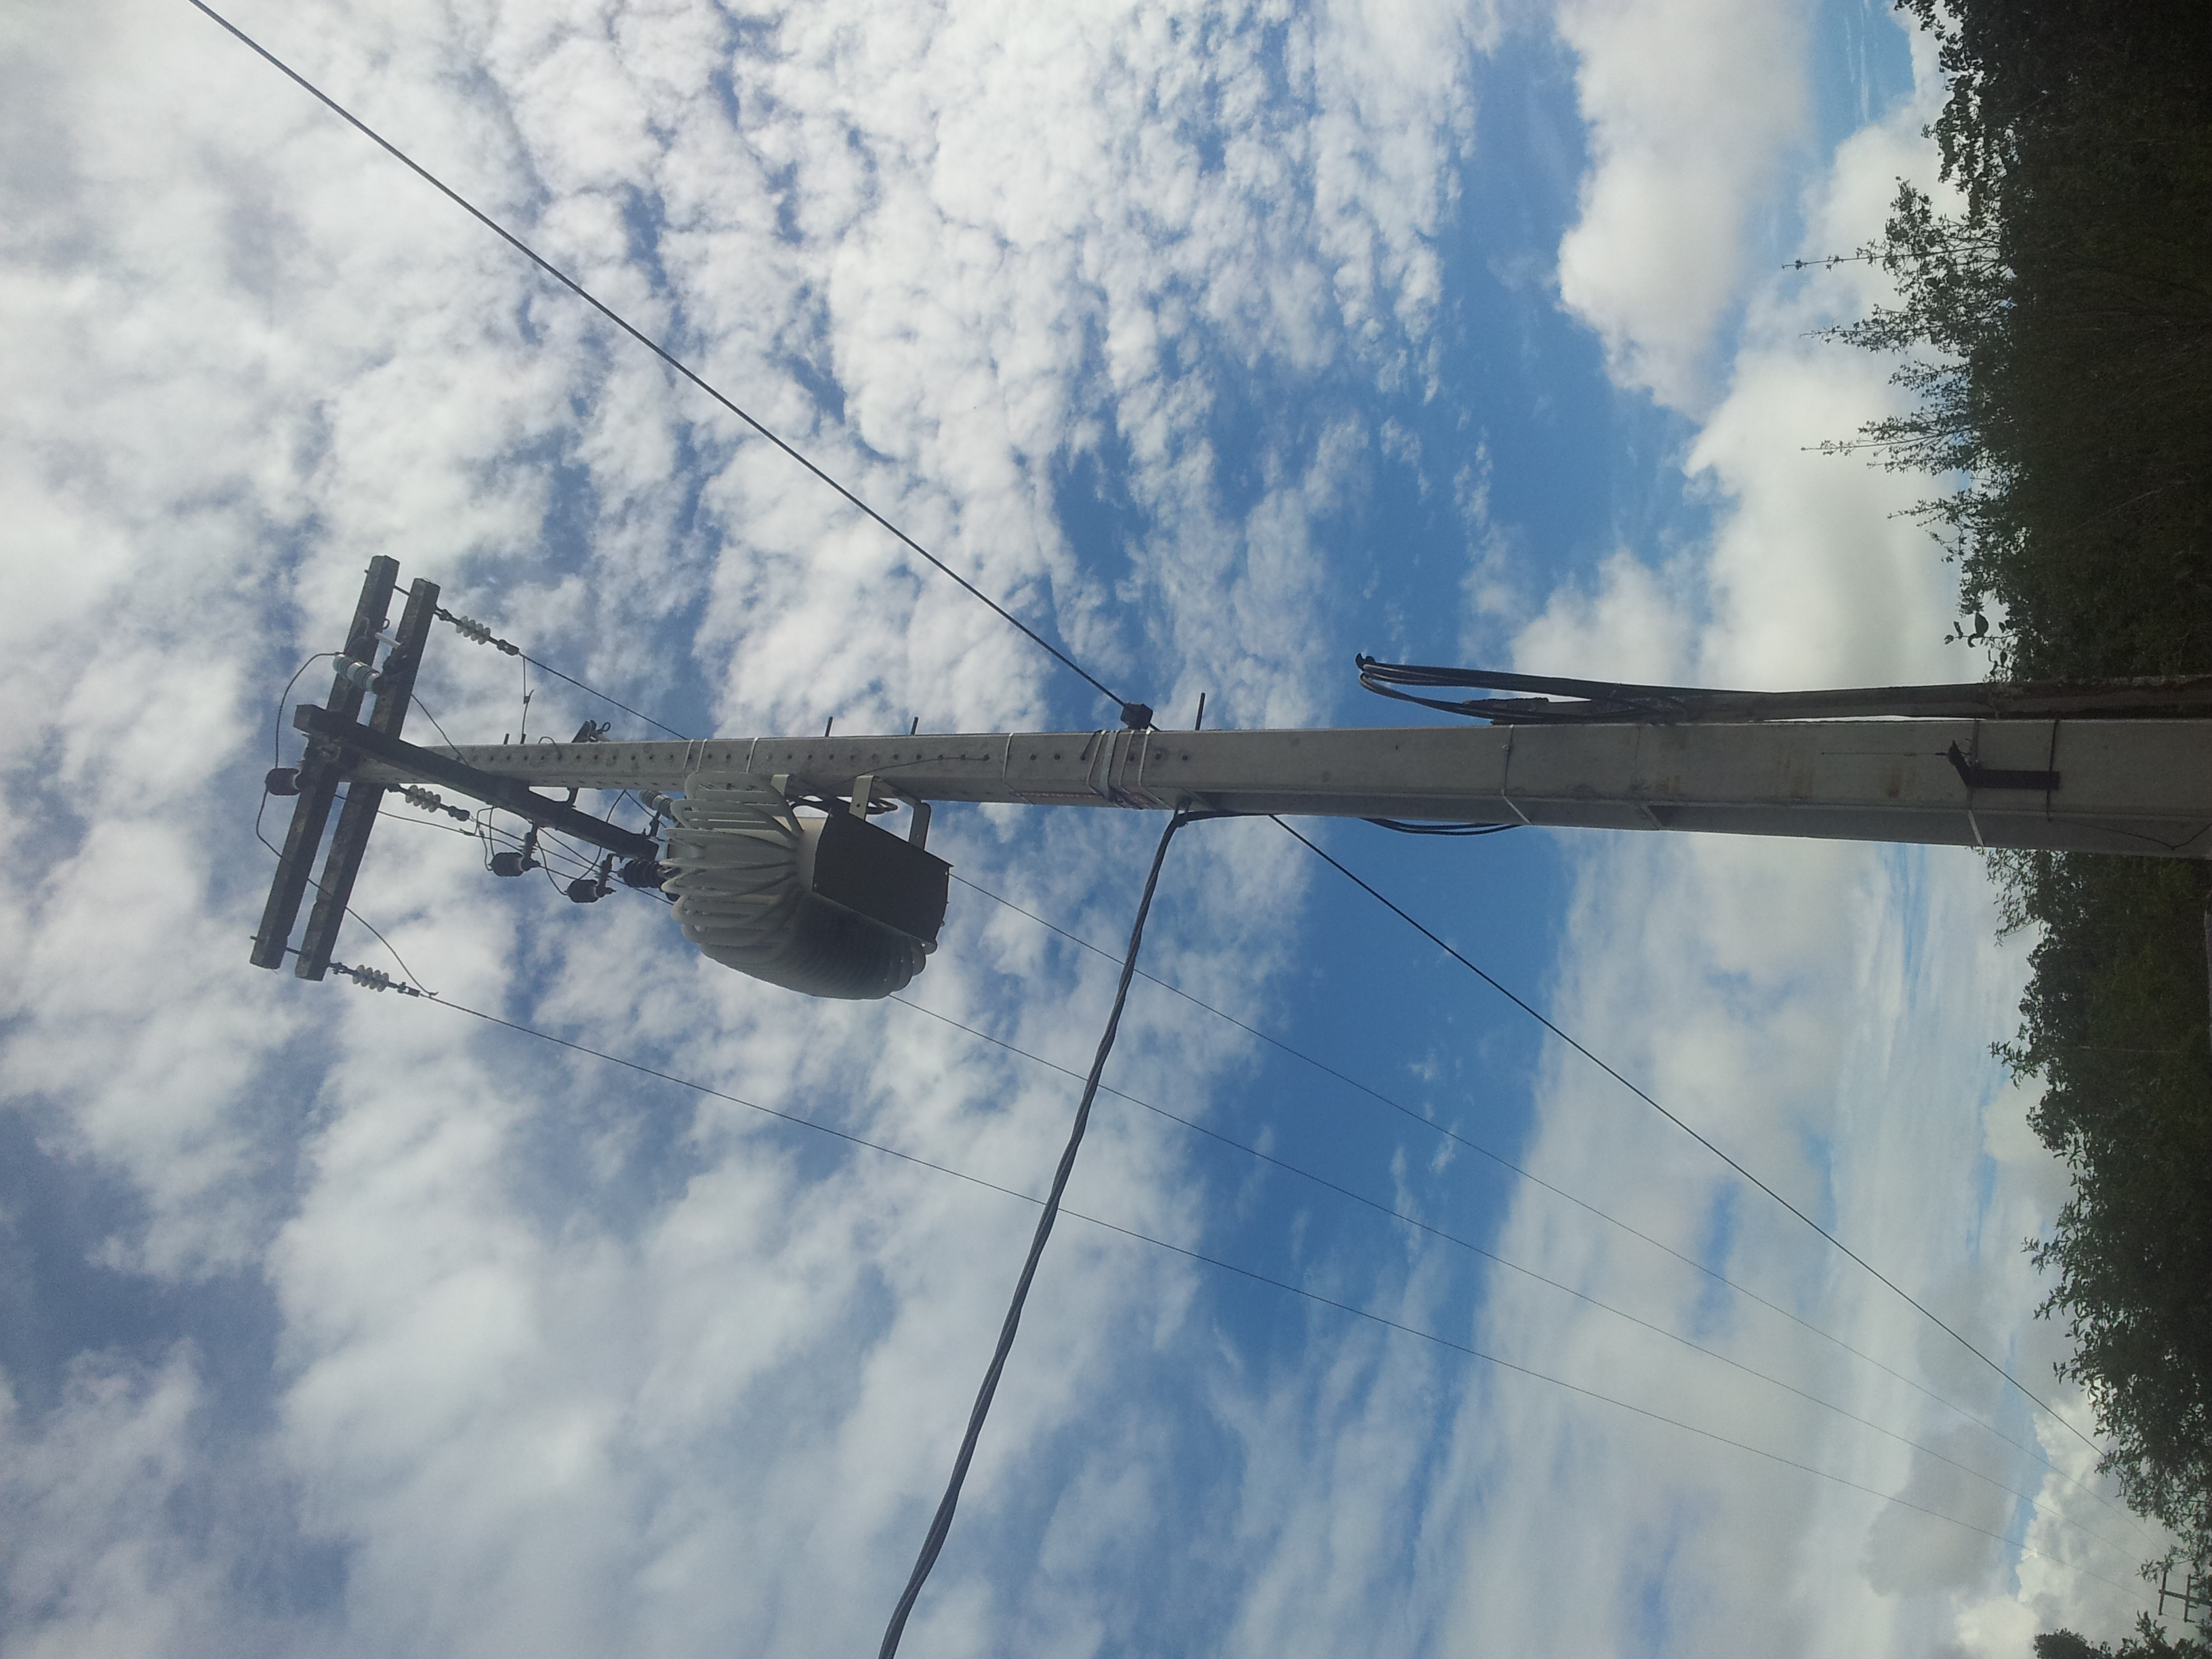
\includegraphics[width=6cm,height=6cm, angle = 270]{./pic/N1_Trafo.jpg}}
\subfloat[Estrutura N1-N3]{
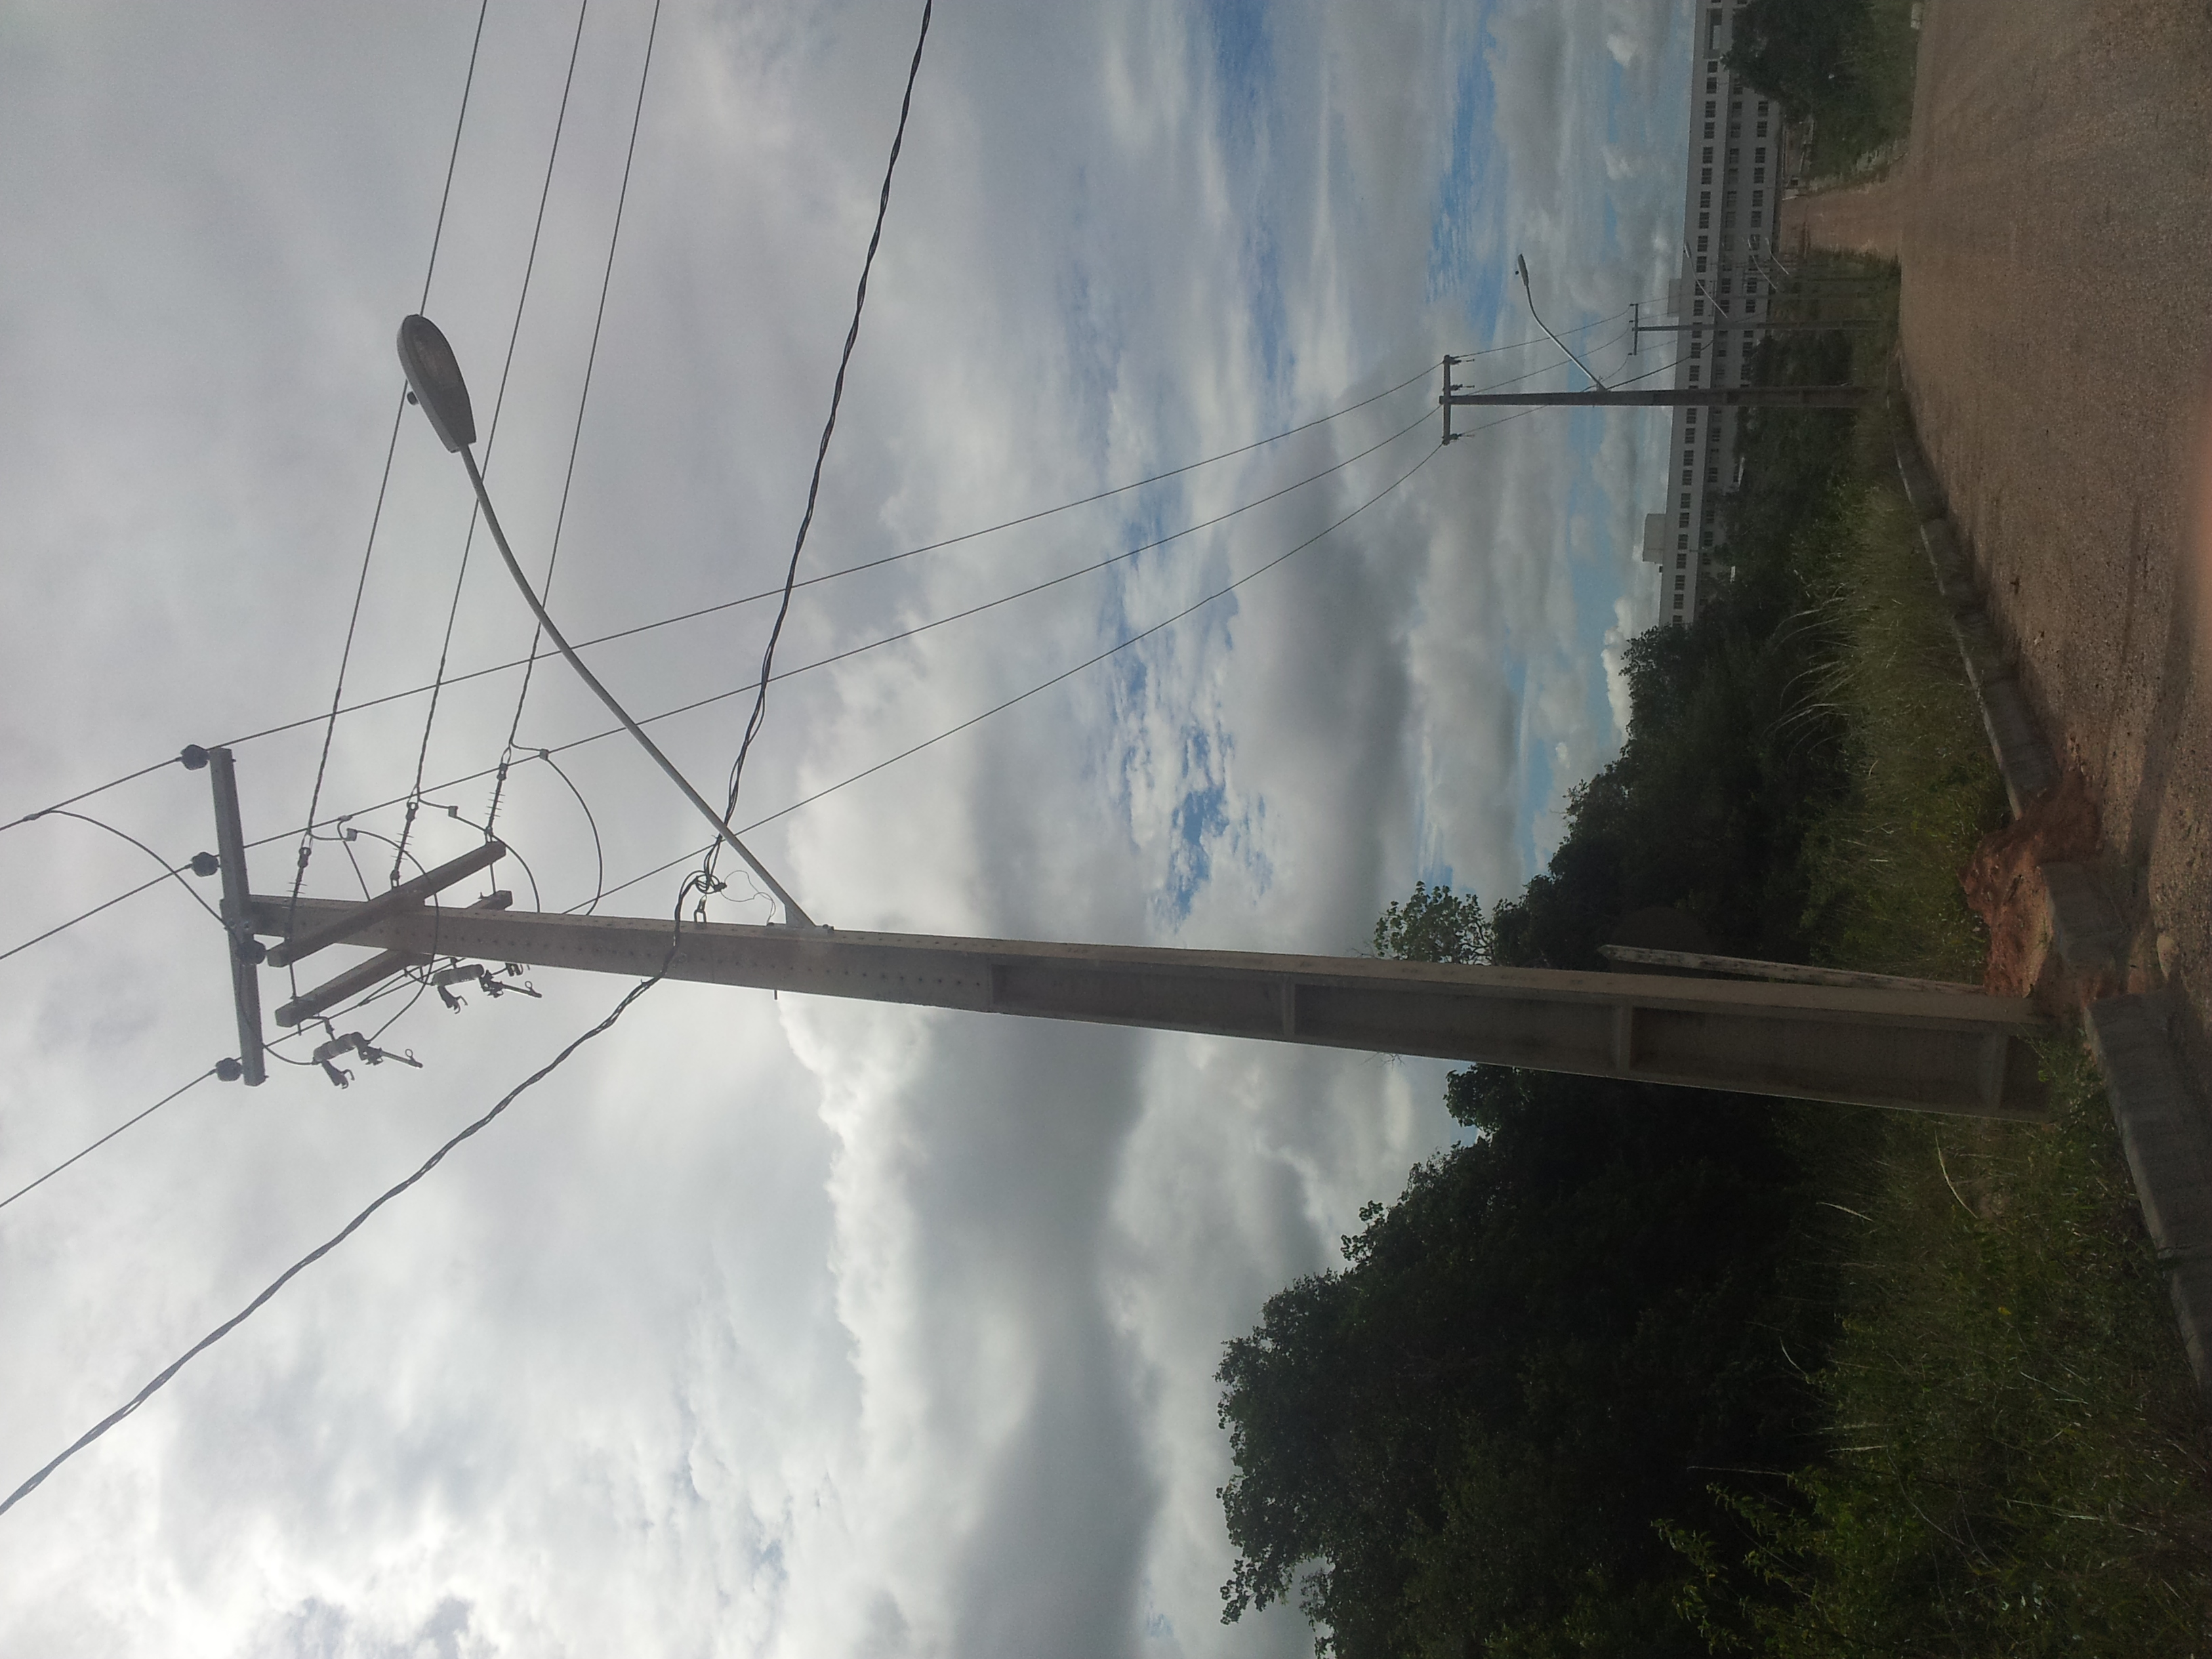
\includegraphics[width=6cm,height=6cm, angle = 270]{./pic/N1N3.jpg}}
\qquad
\subfloat[Estrutura N3-N3, derivação em ângulo fechado]{
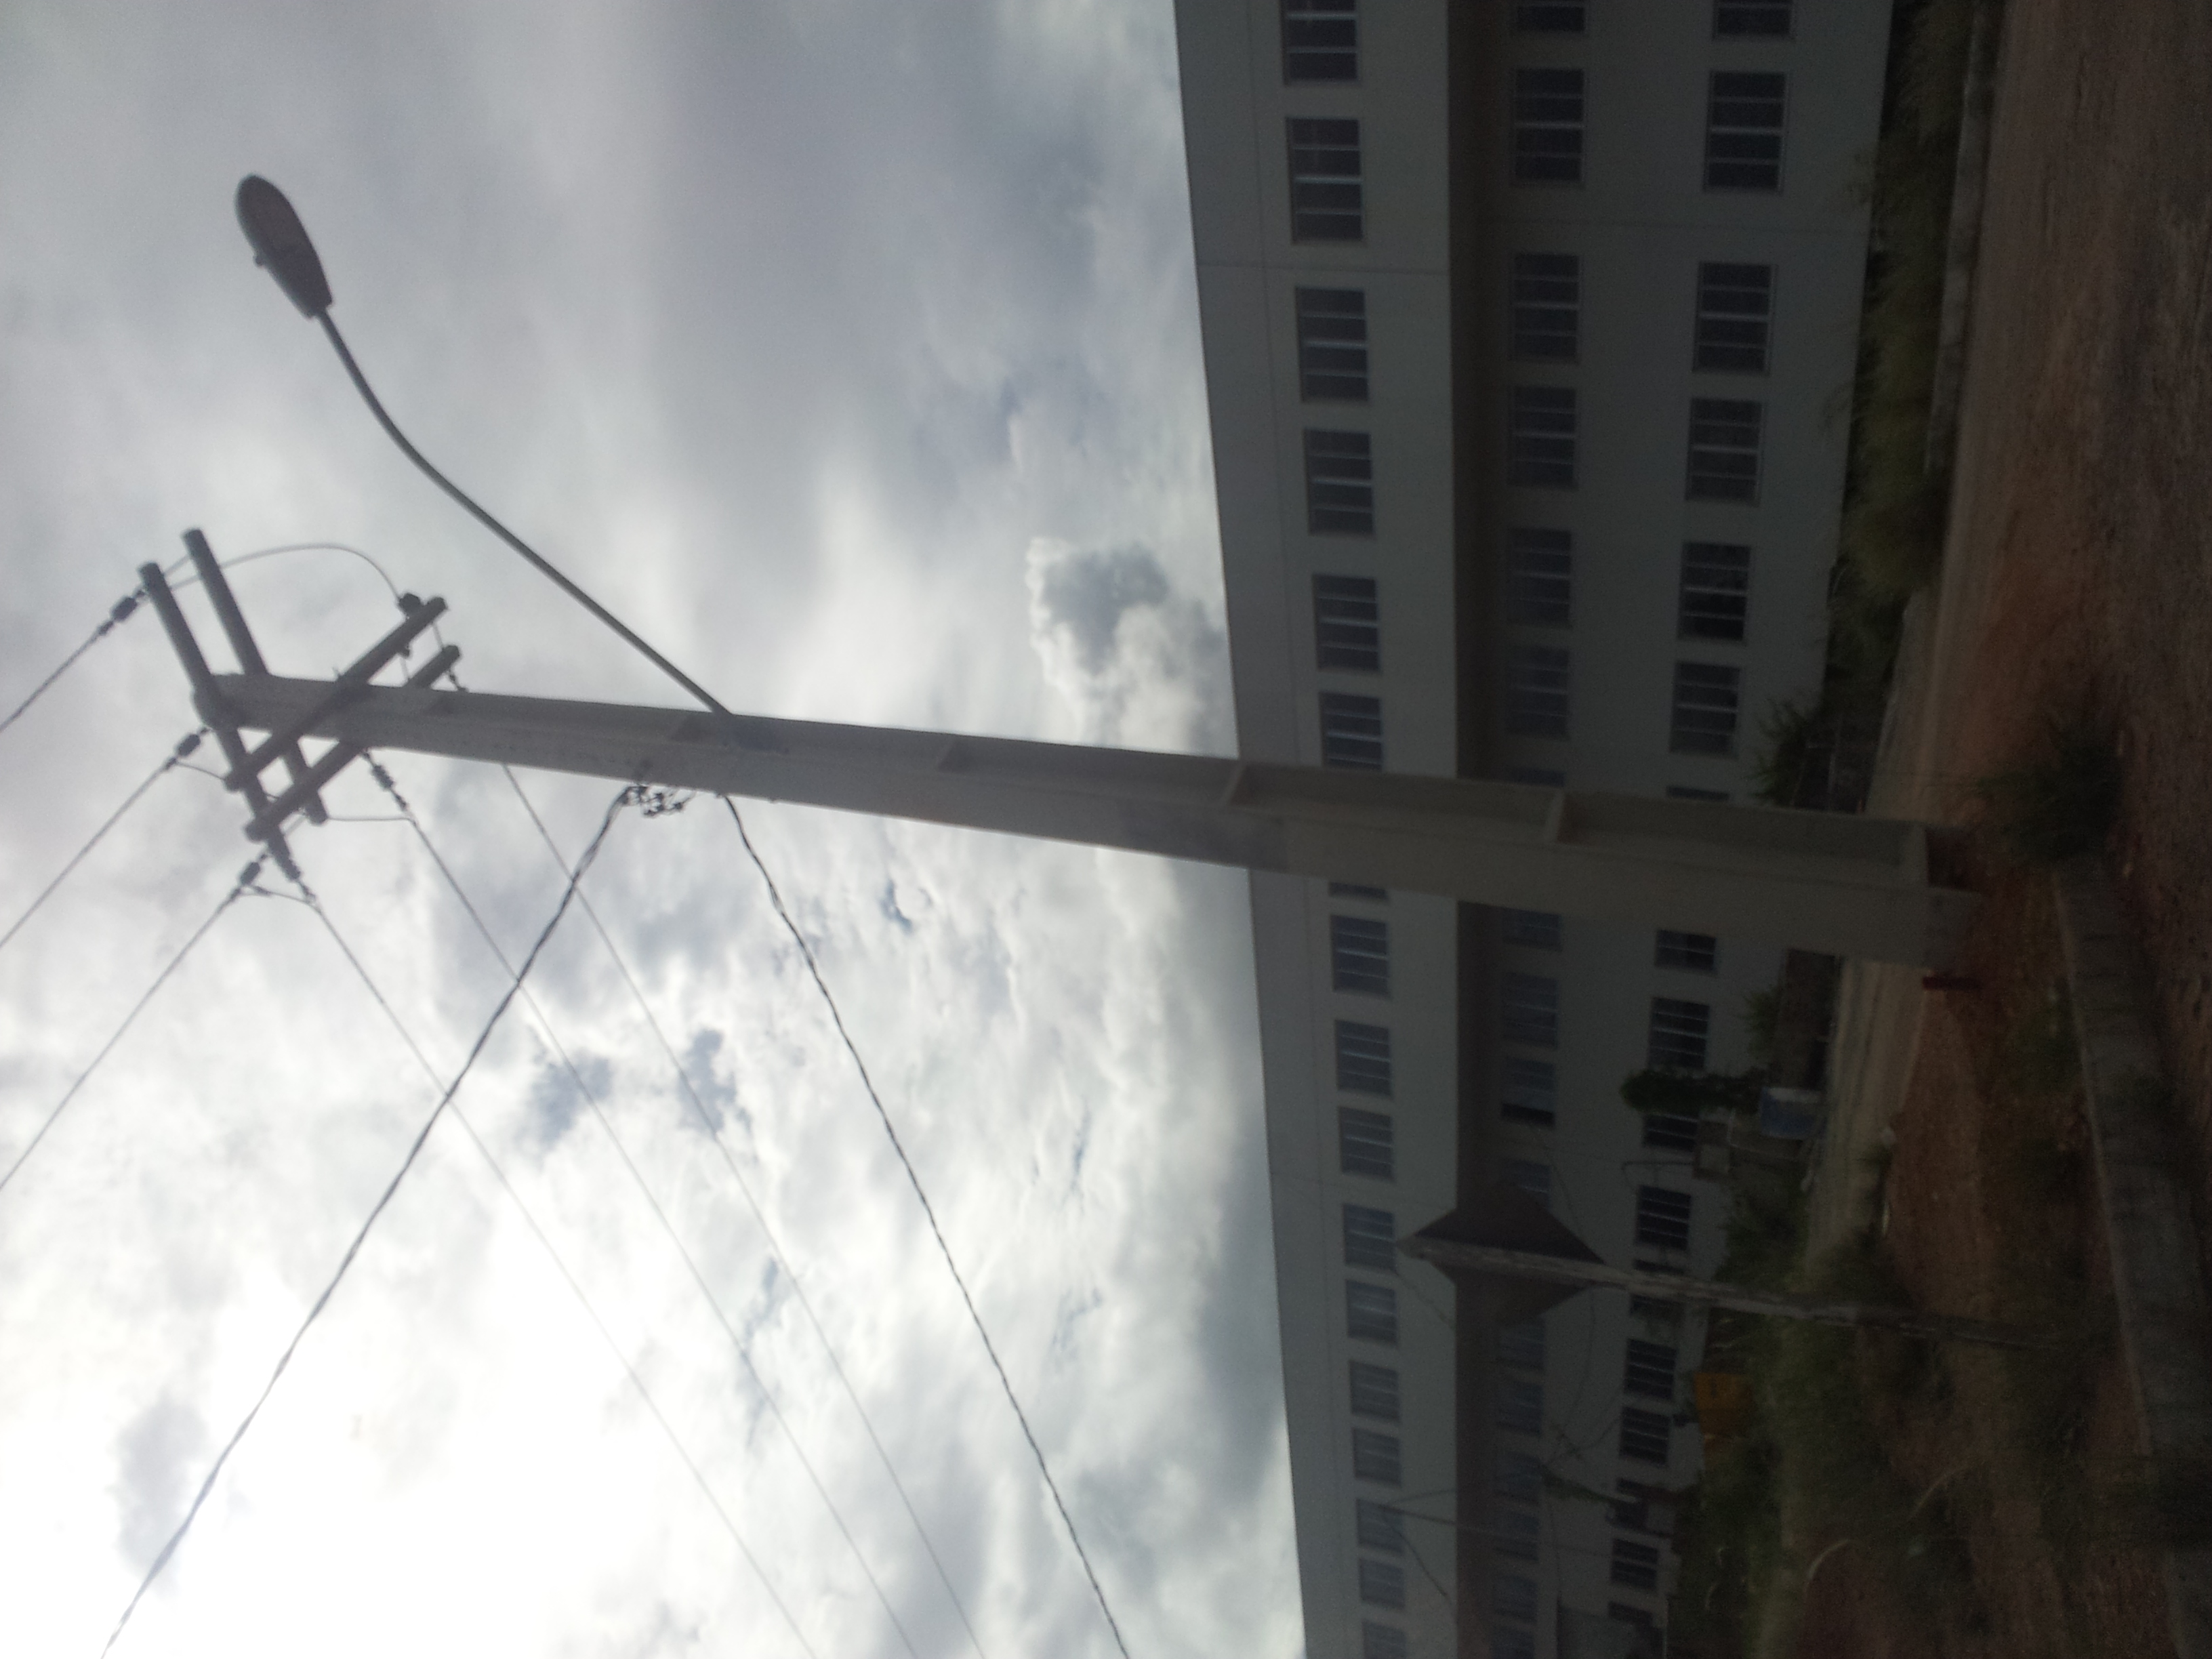
\includegraphics[width=6cm,height=6cm, angle = 270]{./pic/N3N3.jpg}}
\end{figure}

\pagebreak

\subsection{Montagem de Luminária com Munck}

Acompanhei a montagem de luminárias em postes tubulares com a ajuda de braço mecânico montado em caminhão, tirando algumas fotos do procedimento. Antes de fazer a montagem é necessária a escavação de valas subterrâneas, colocação de caixas de passagem e eletrodutos com cabo guia que serve para puxar os fios. A instalação é subterrânea pois no caso da iluminação em edifícios públicos tem se adotado cada vez mais o cabeamento subterrâneo devido a razões estéticas. O processo está fotografado nas figuras de letra "m" até "r" 

\begin{figure}
\ContinuedFloat
\centering
\subfloat[Vala com Eletroduto]{
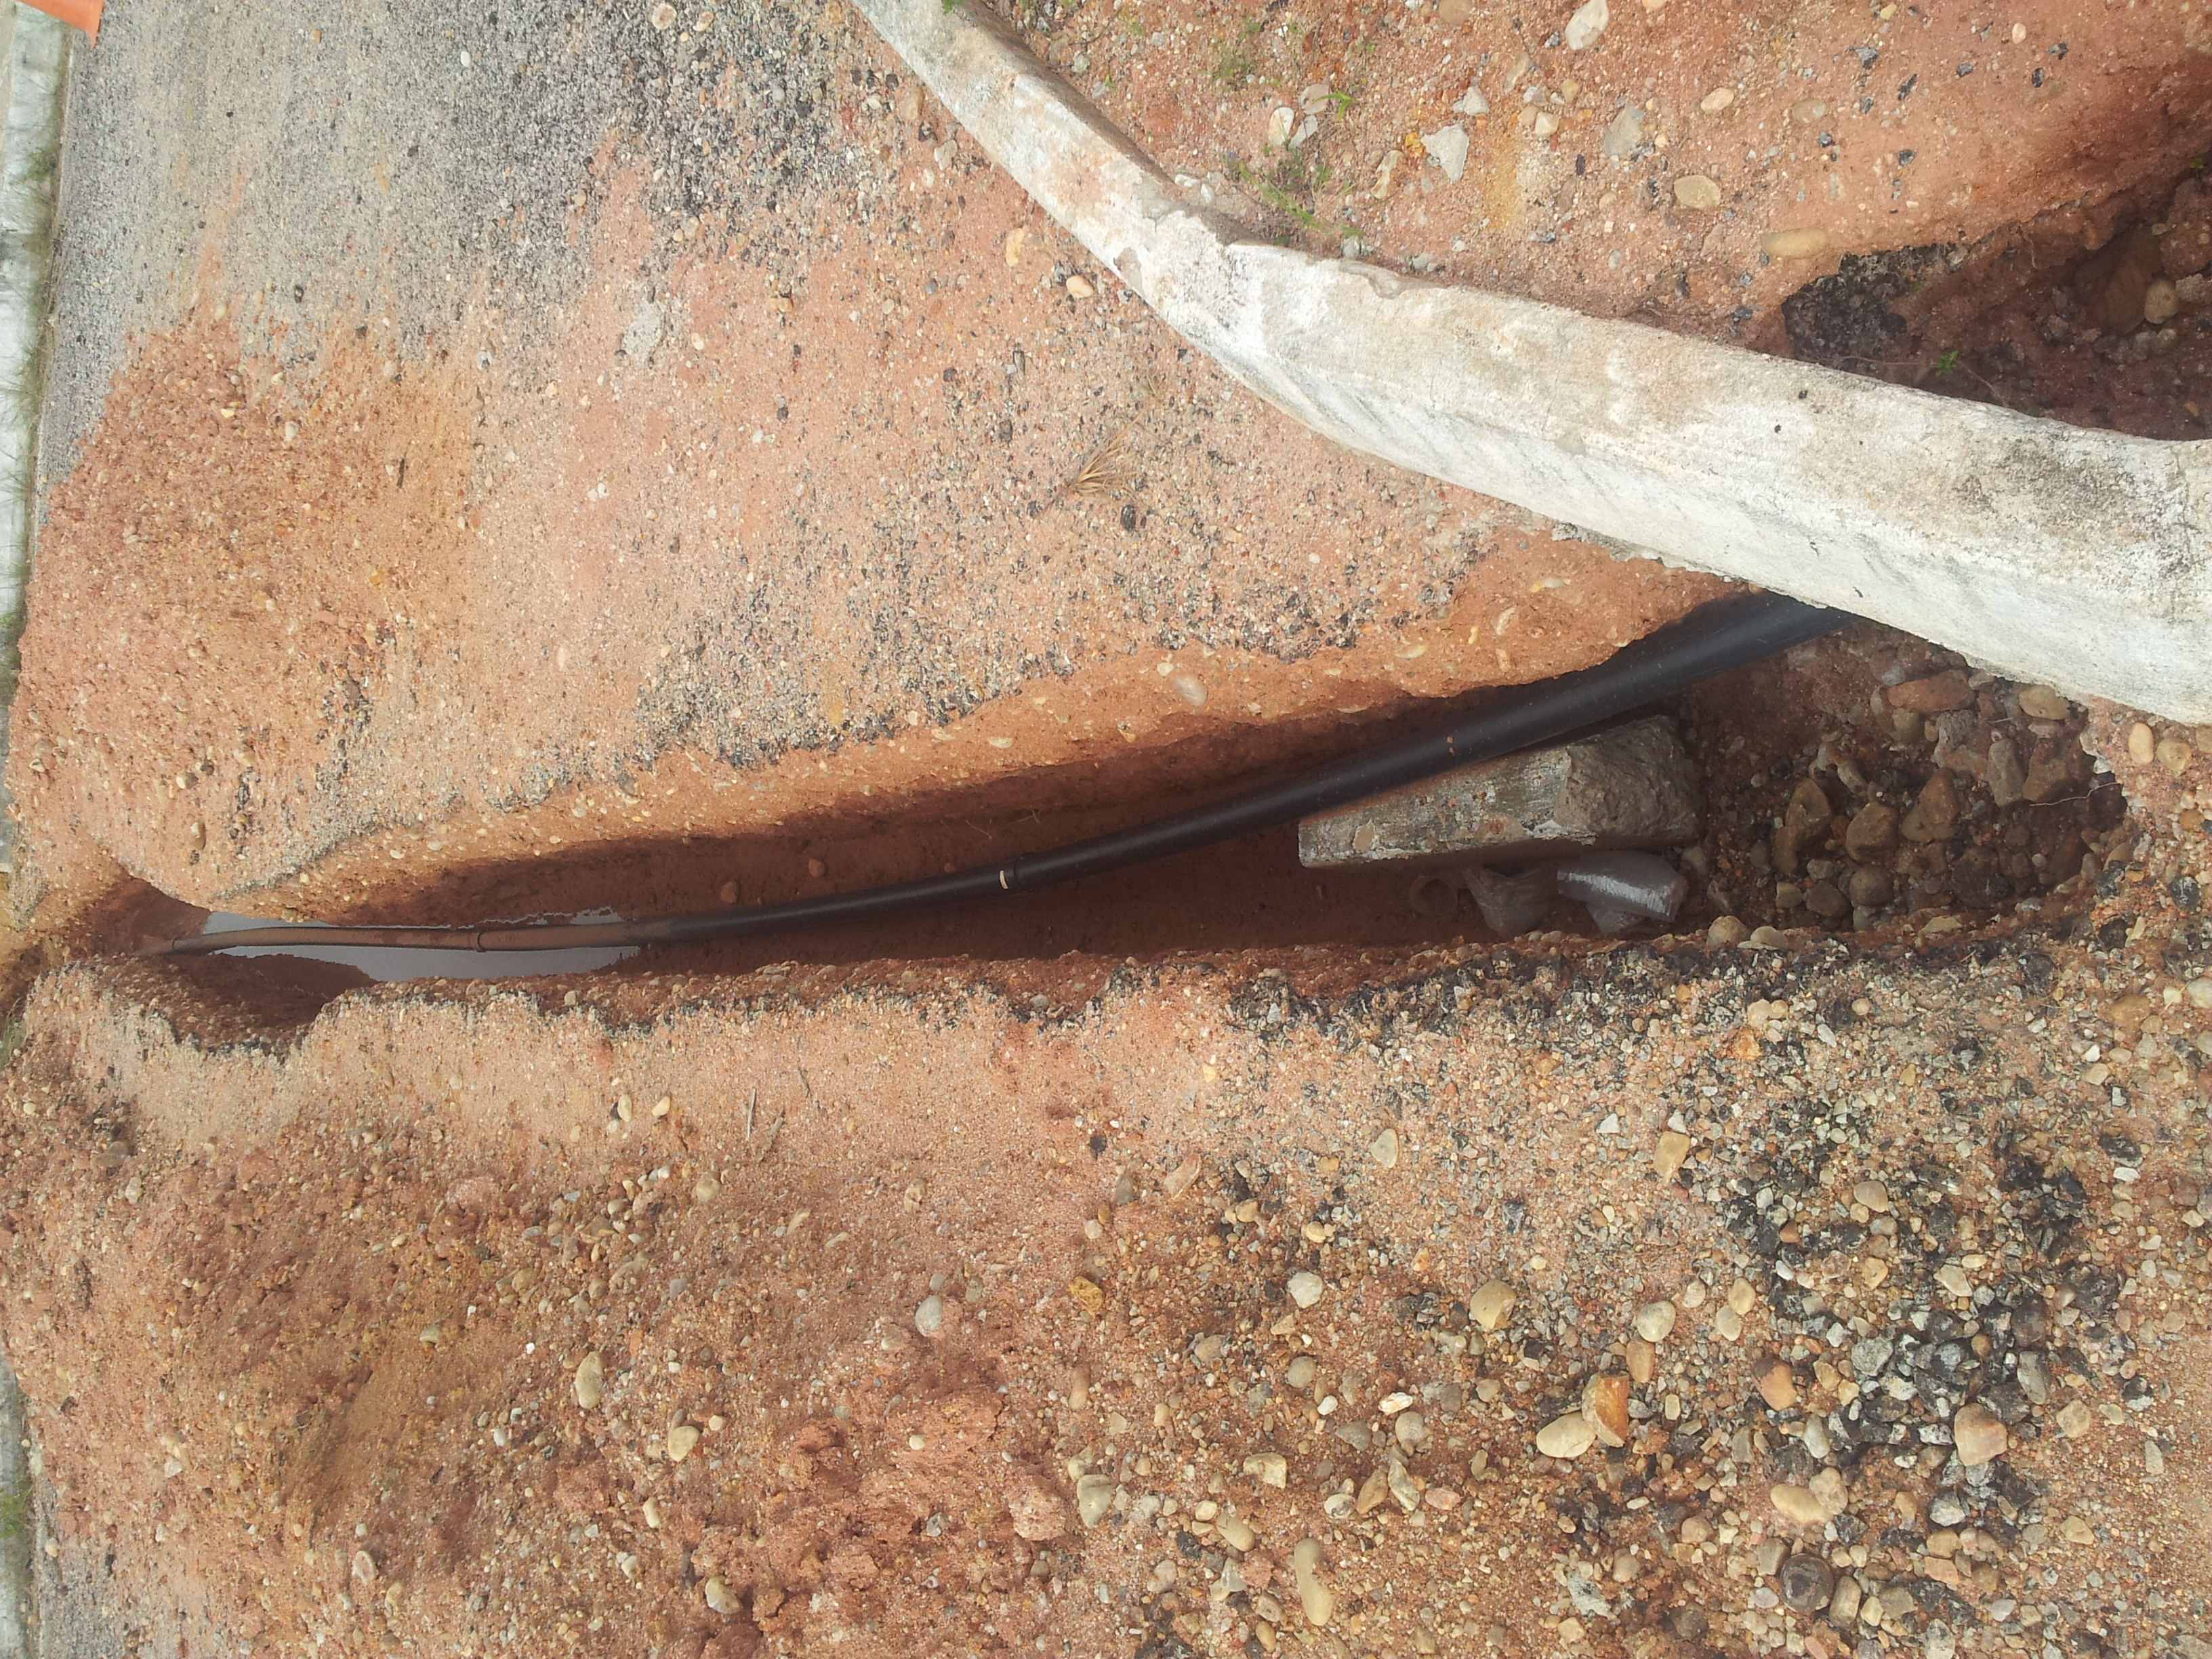
\includegraphics[width=4cm,height=4cm, angle = 270]{./pic/ValaPassagem.jpg}}
\subfloat[Caixa de Passagem]{
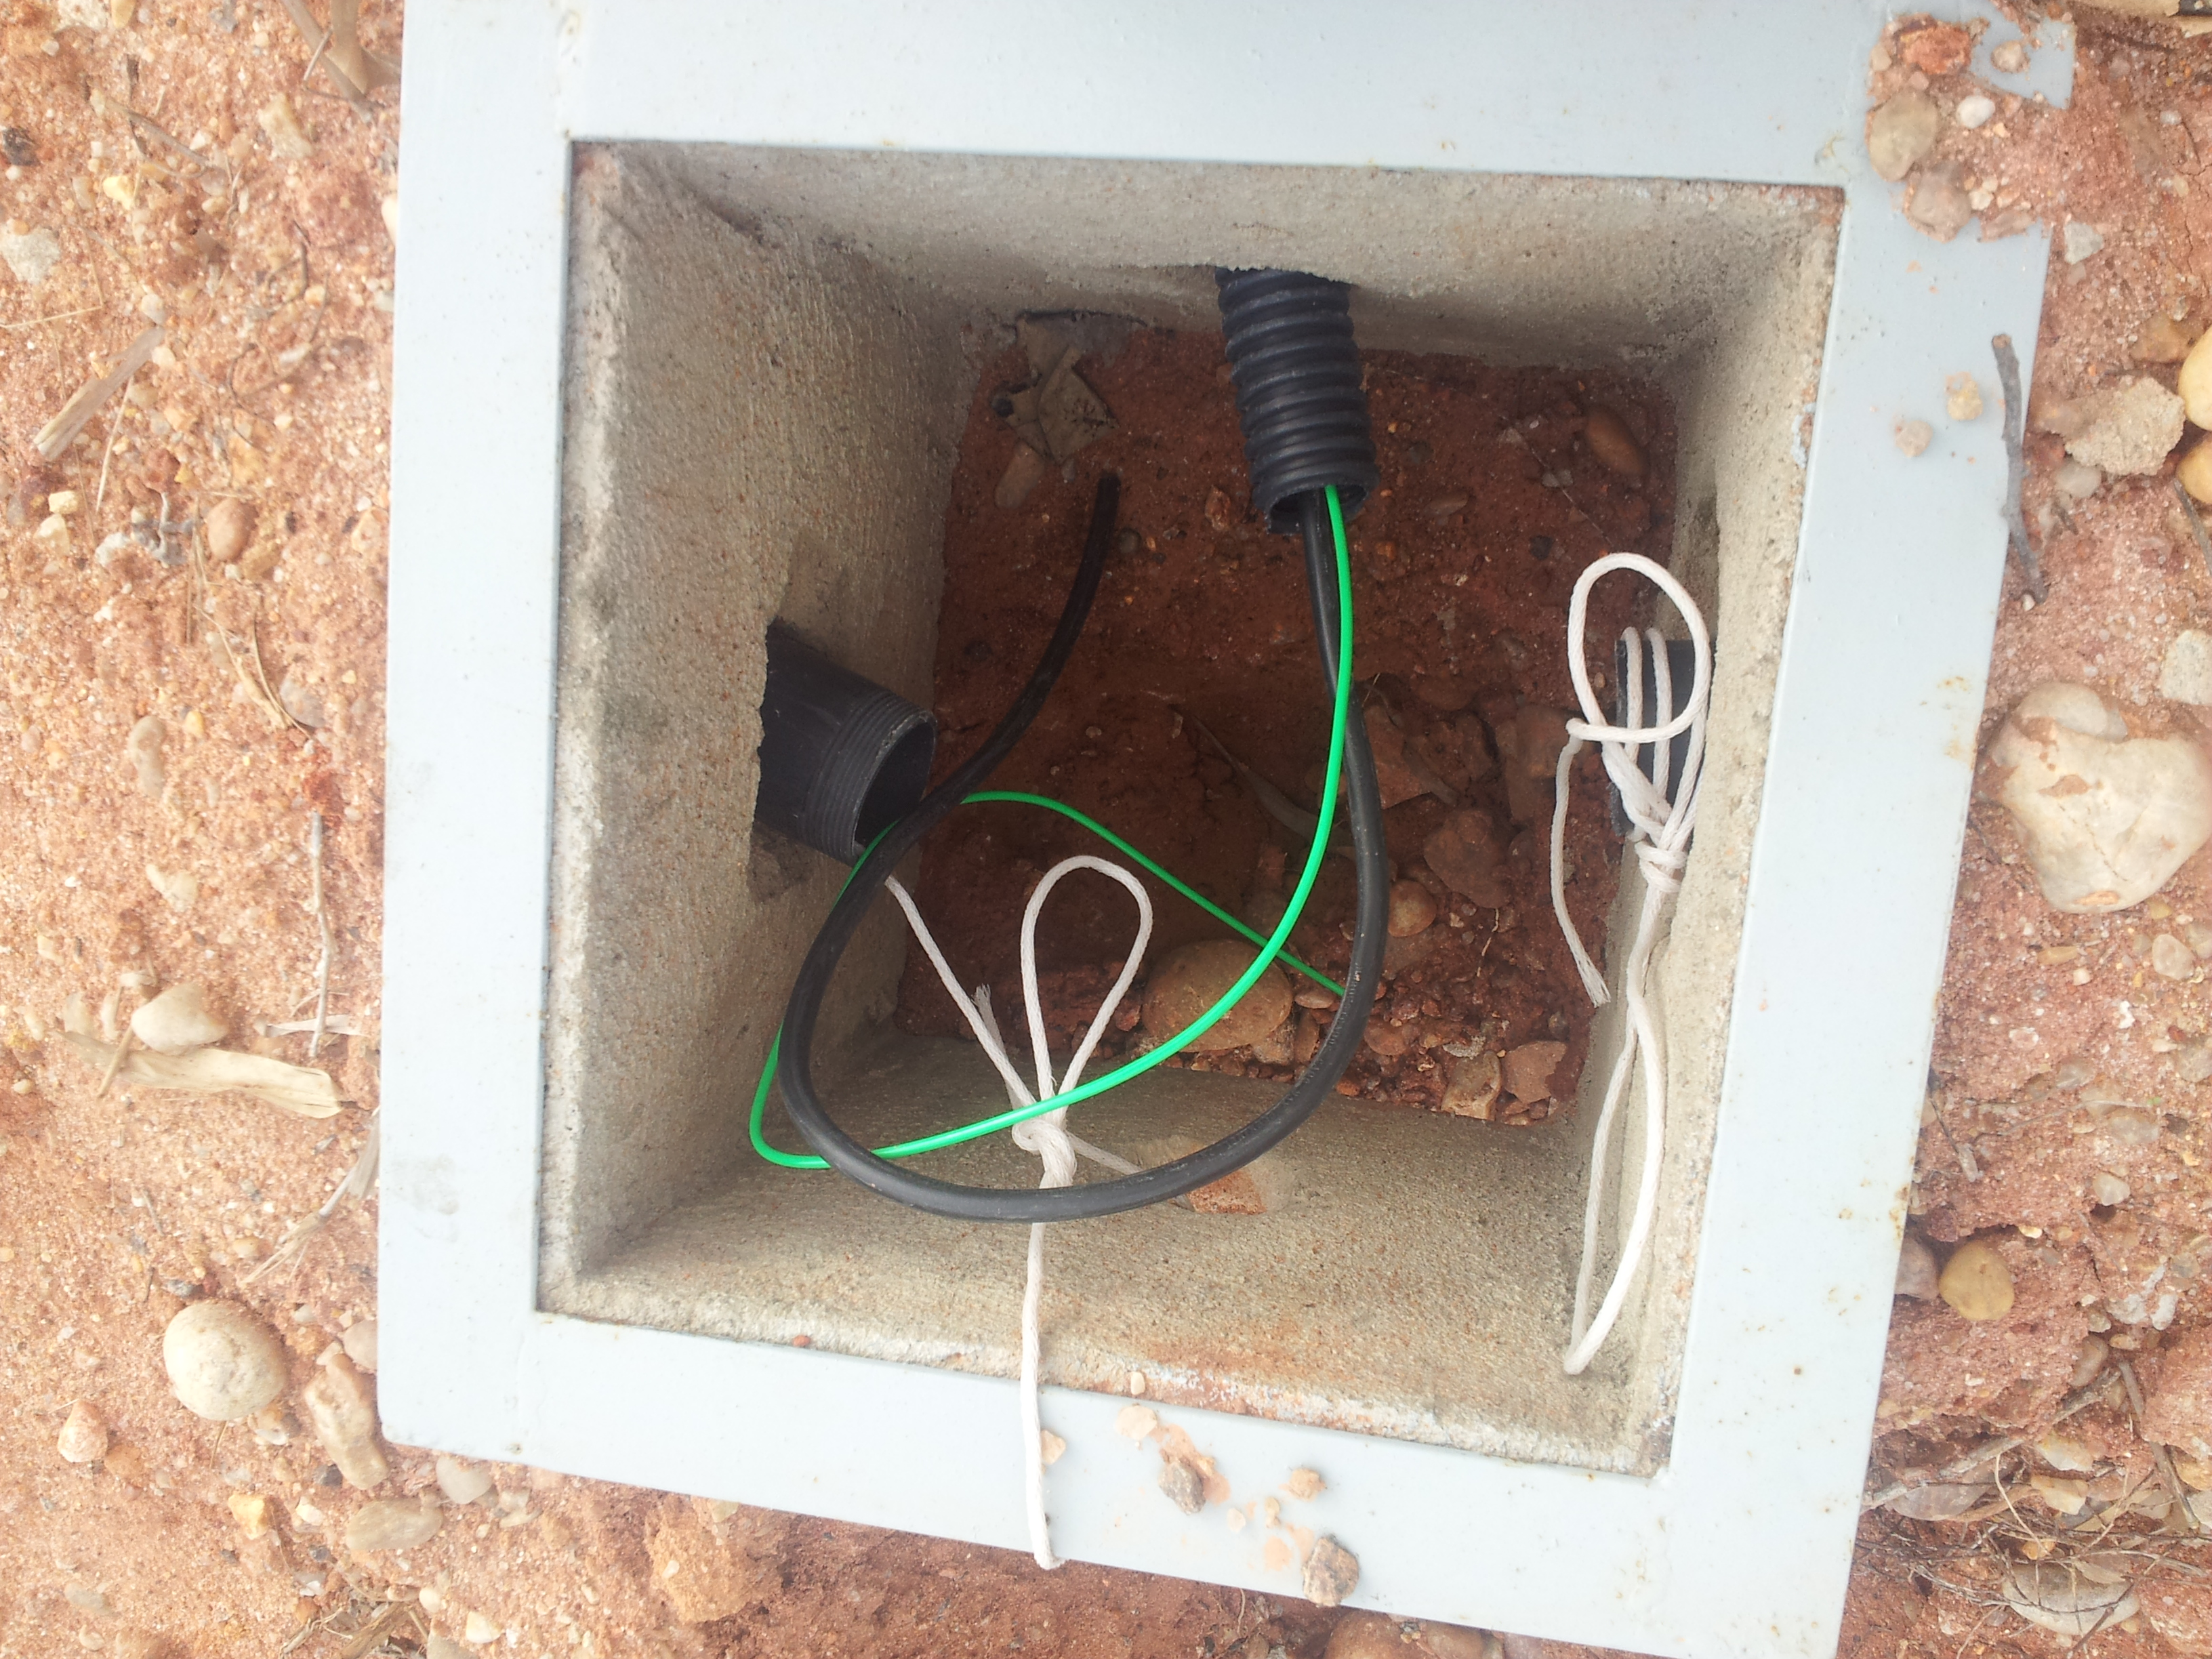
\includegraphics[width=4cm,height=4cm, angle = 270]{./pic/CxPassagem.jpg}}
\subfloat[Luminárias com Foto Sensores(Amarelo)]{
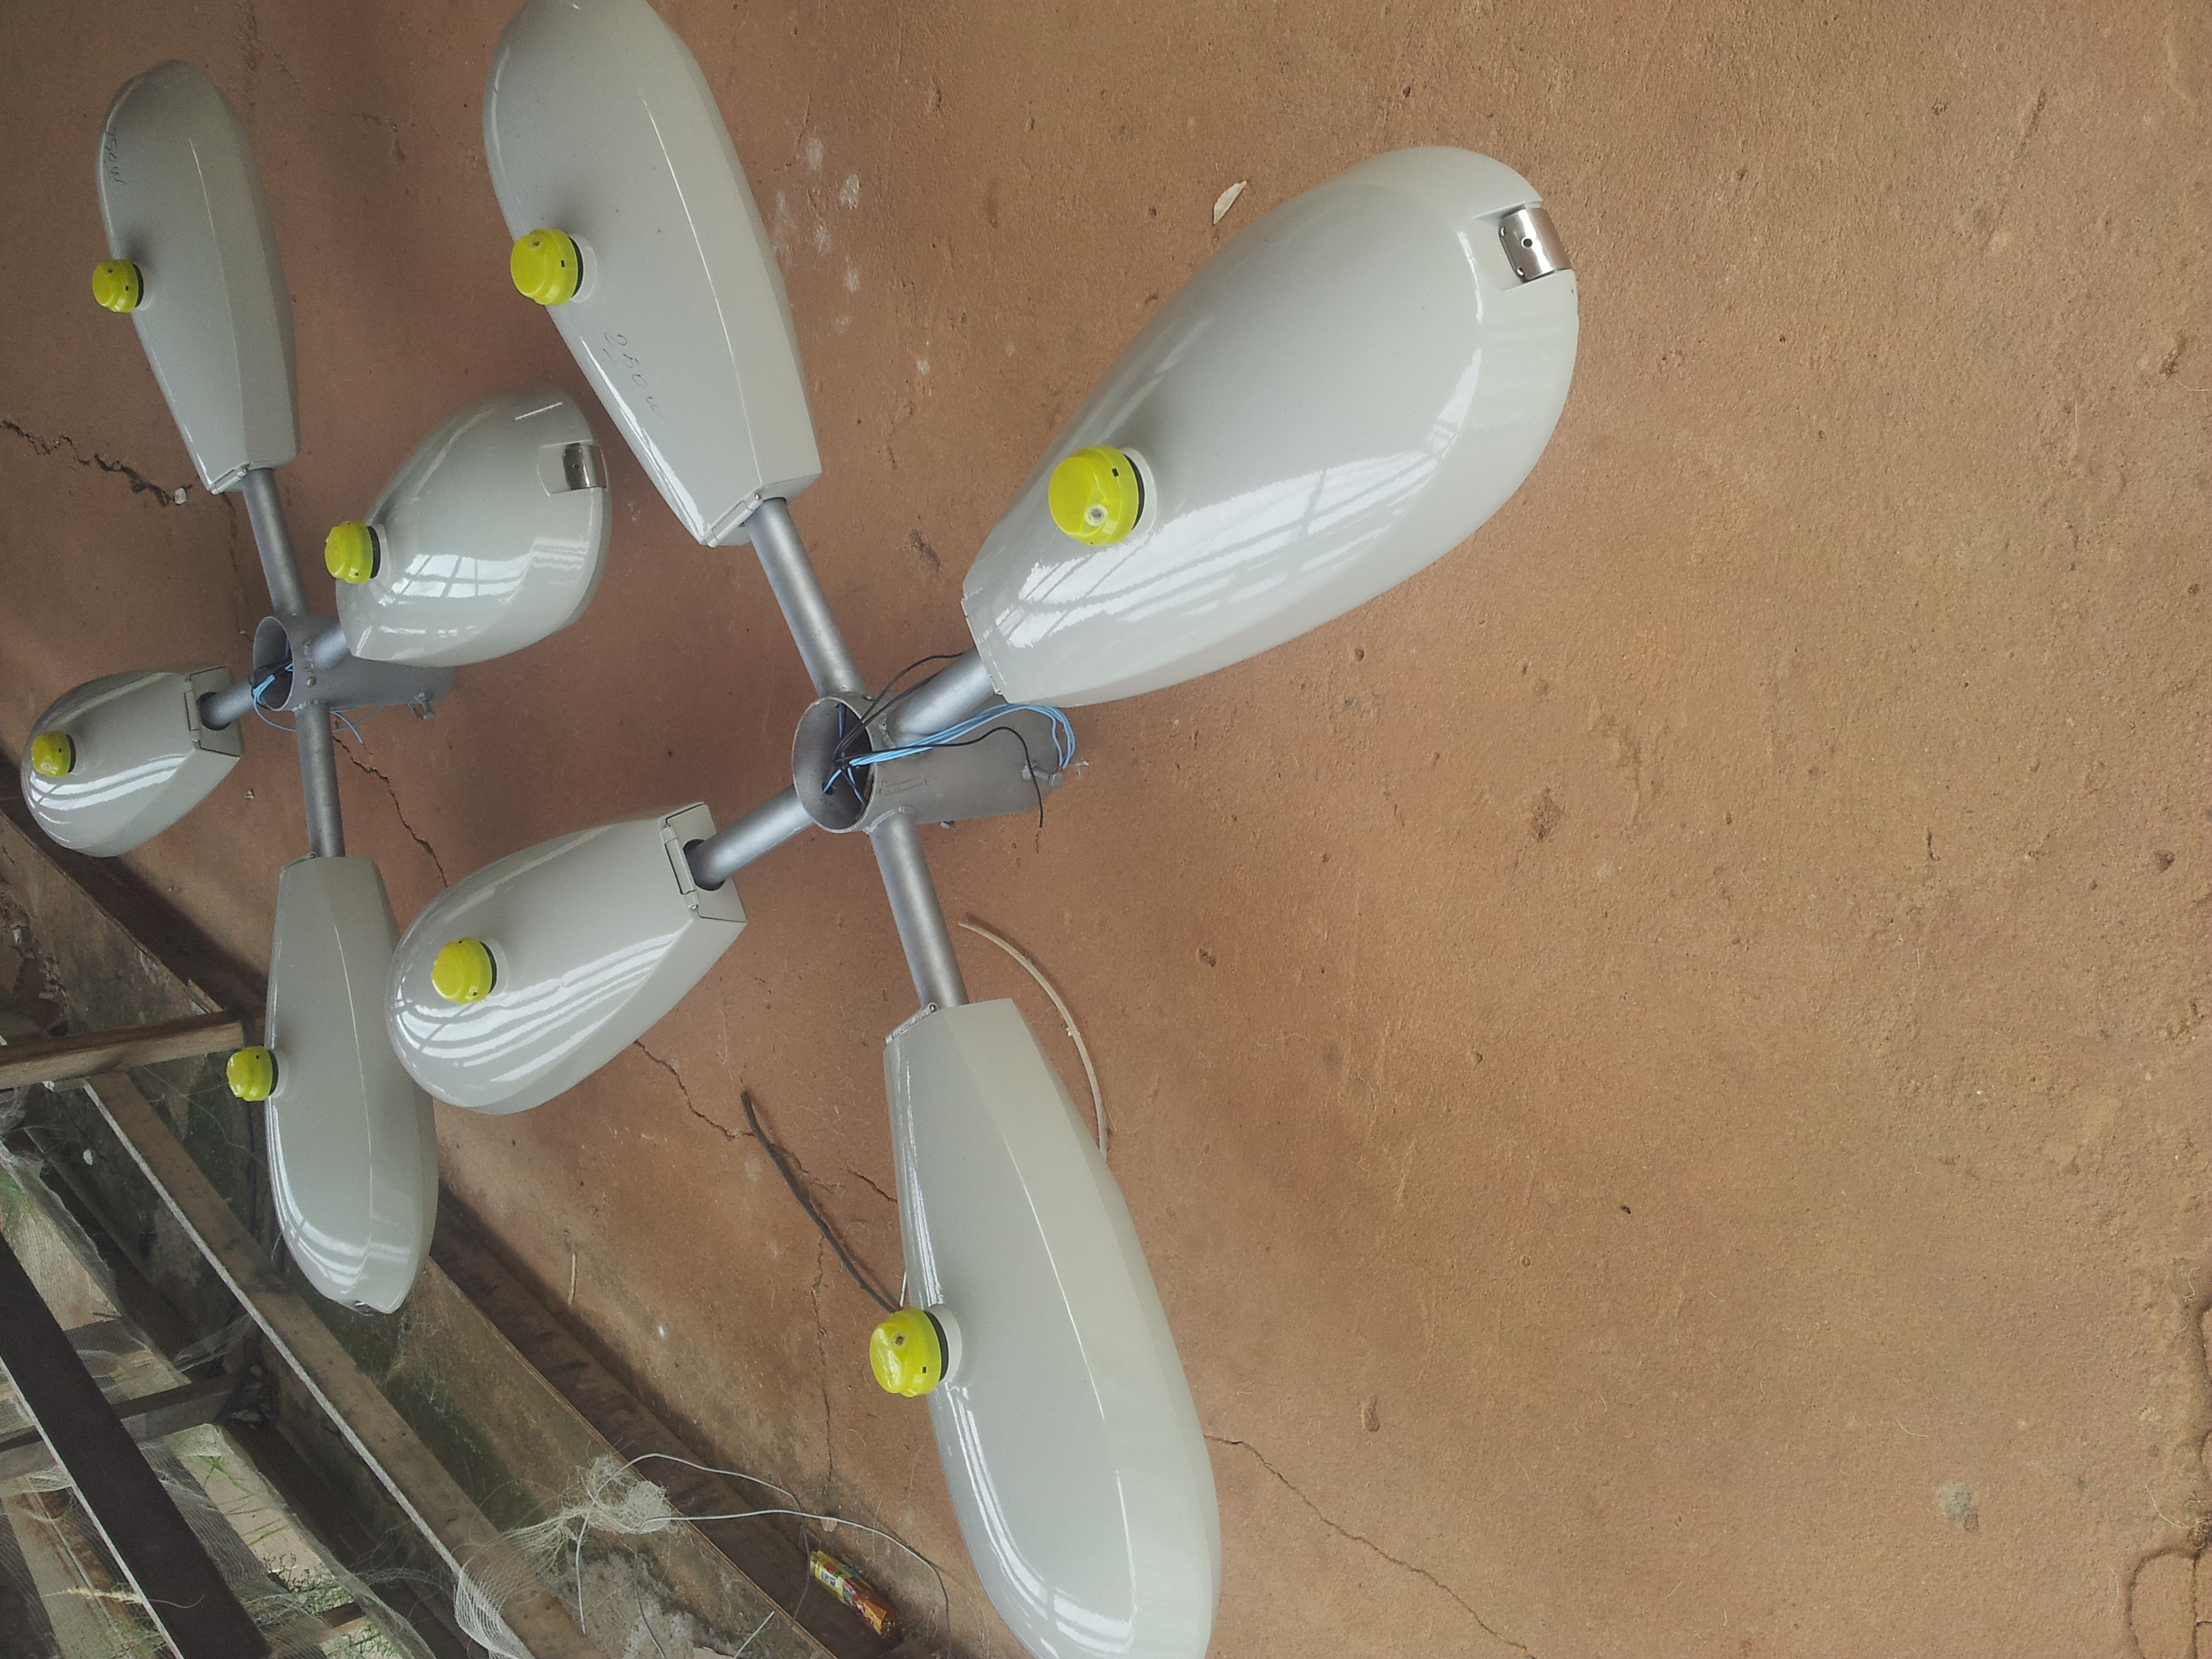
\includegraphics[width=4cm,height=4cm, angle = 270]{./pic/4Petala.jpg}}
\qquad
\subfloat[Munck]{
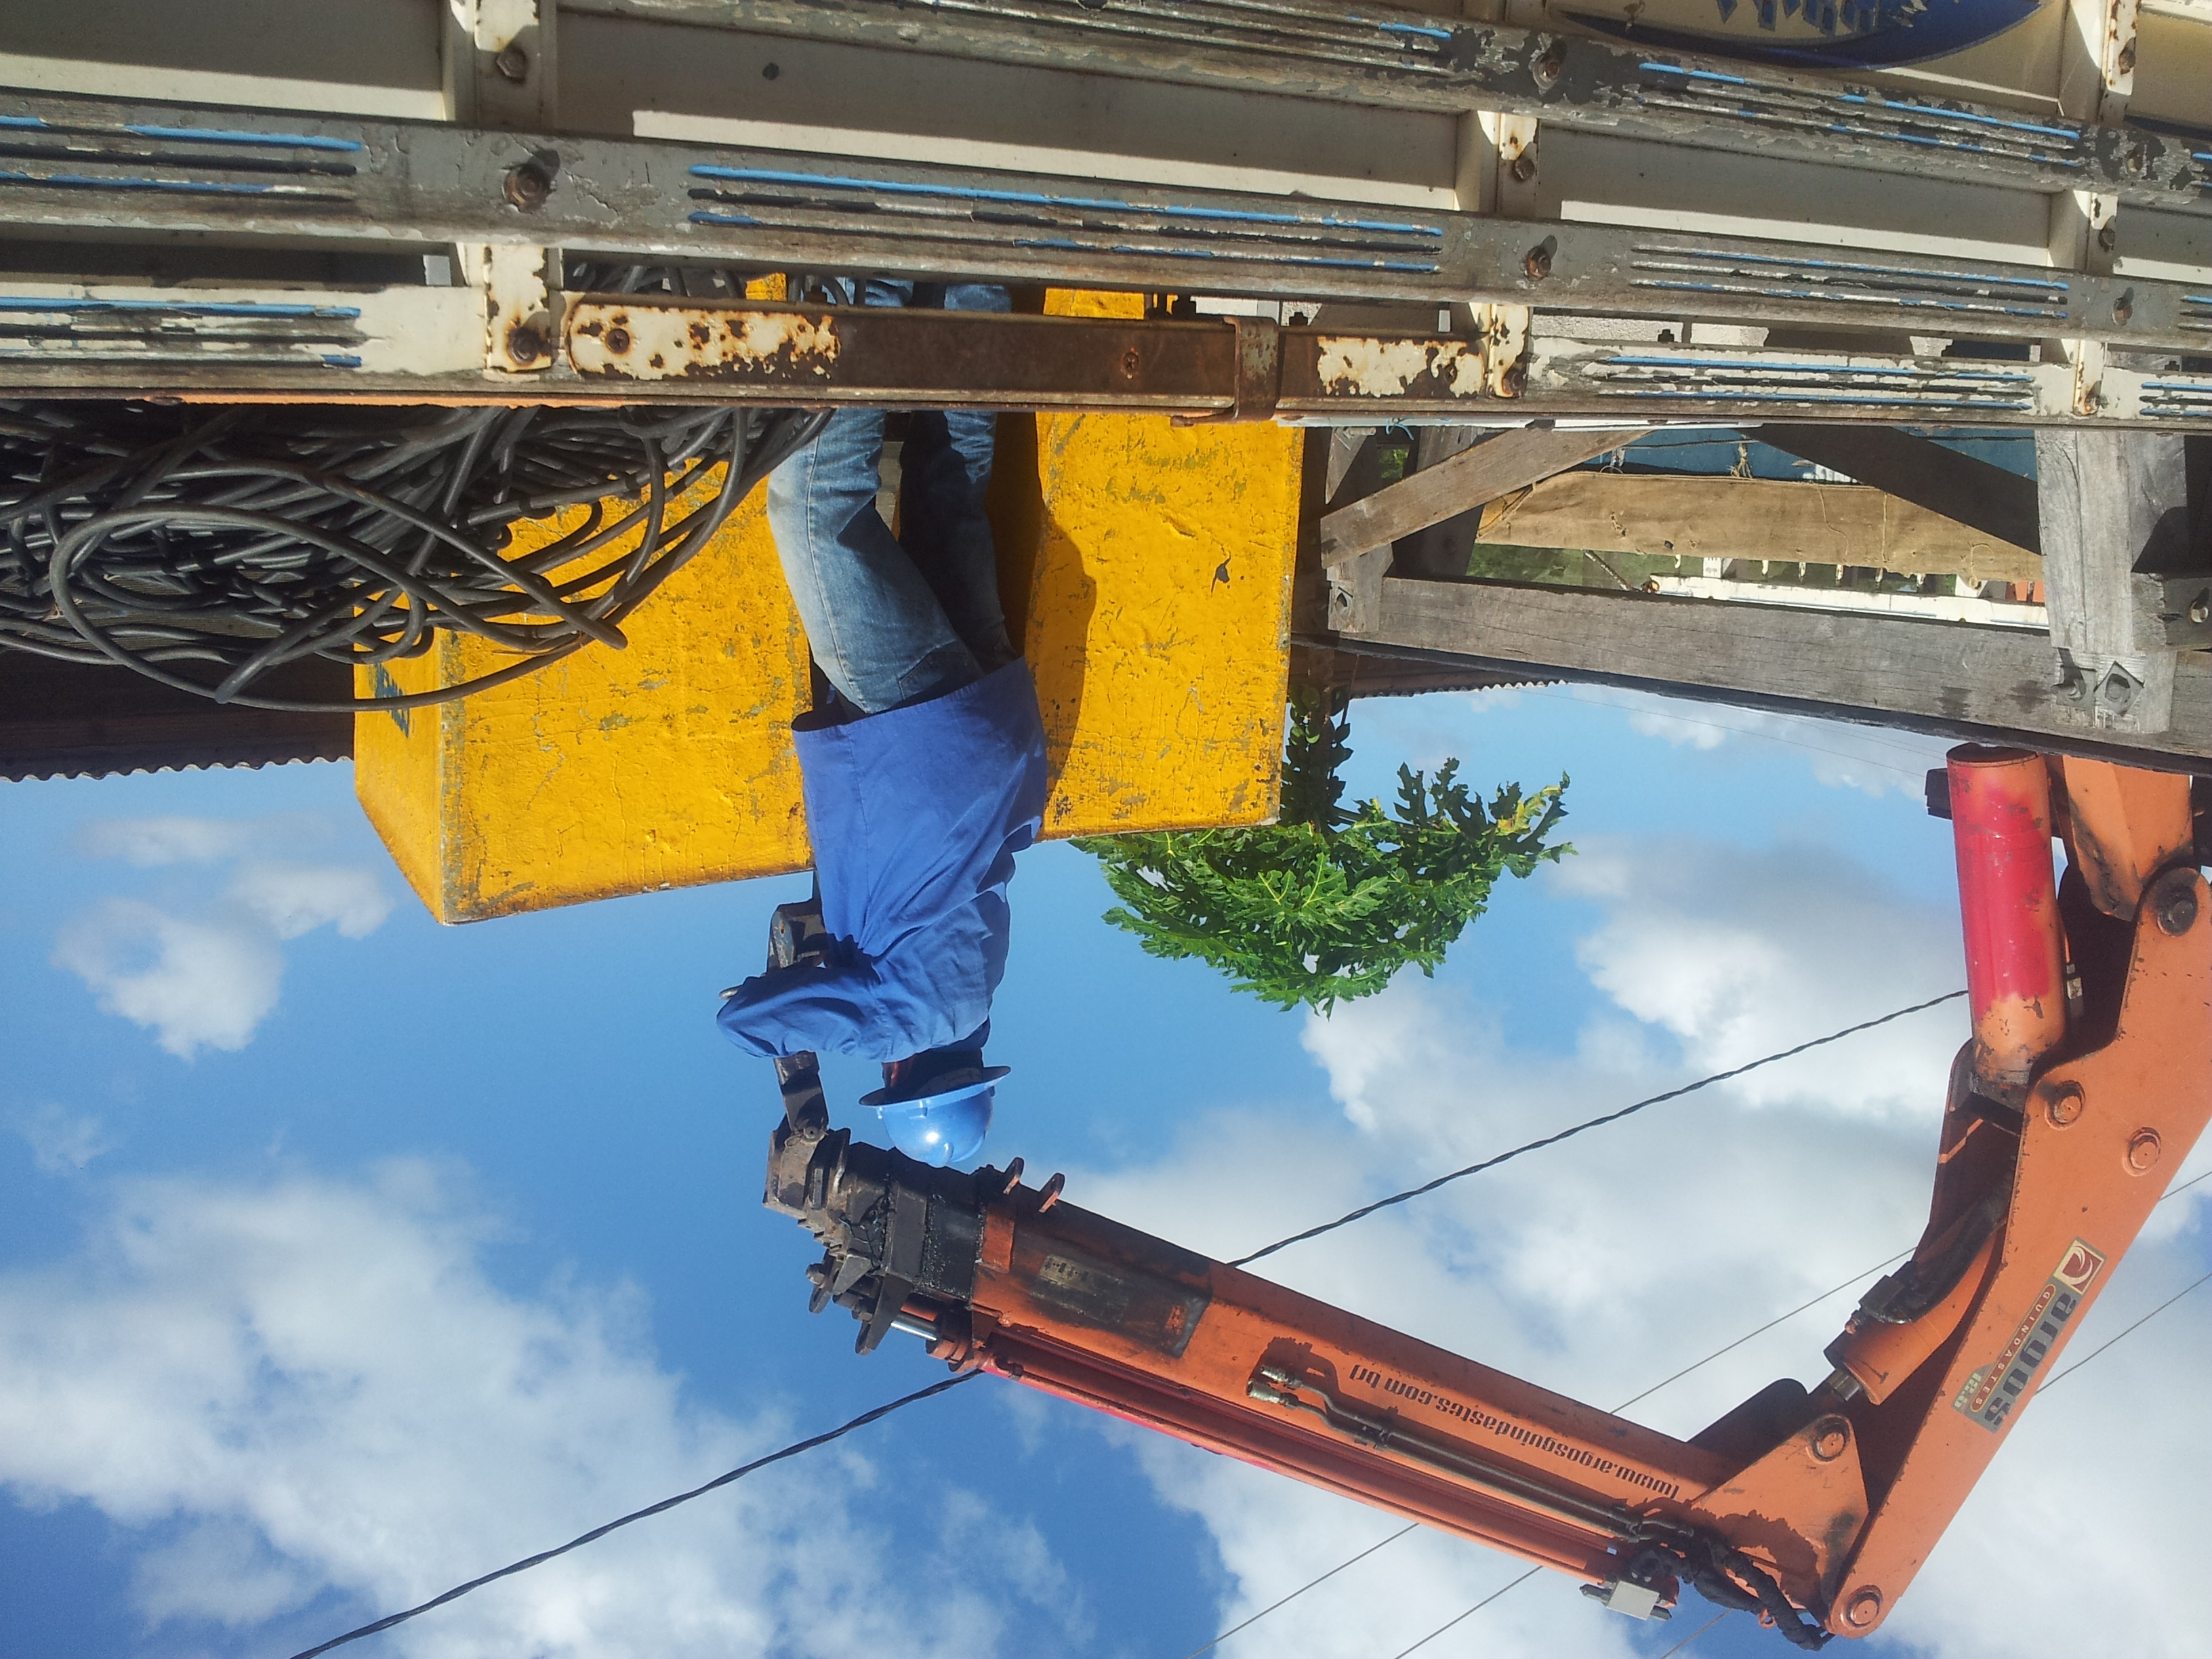
\includegraphics[width=4cm,height=4cm, angle = 180]{./pic/Muck1.jpg}}
\subfloat[Detalhe da terminação do braço]{
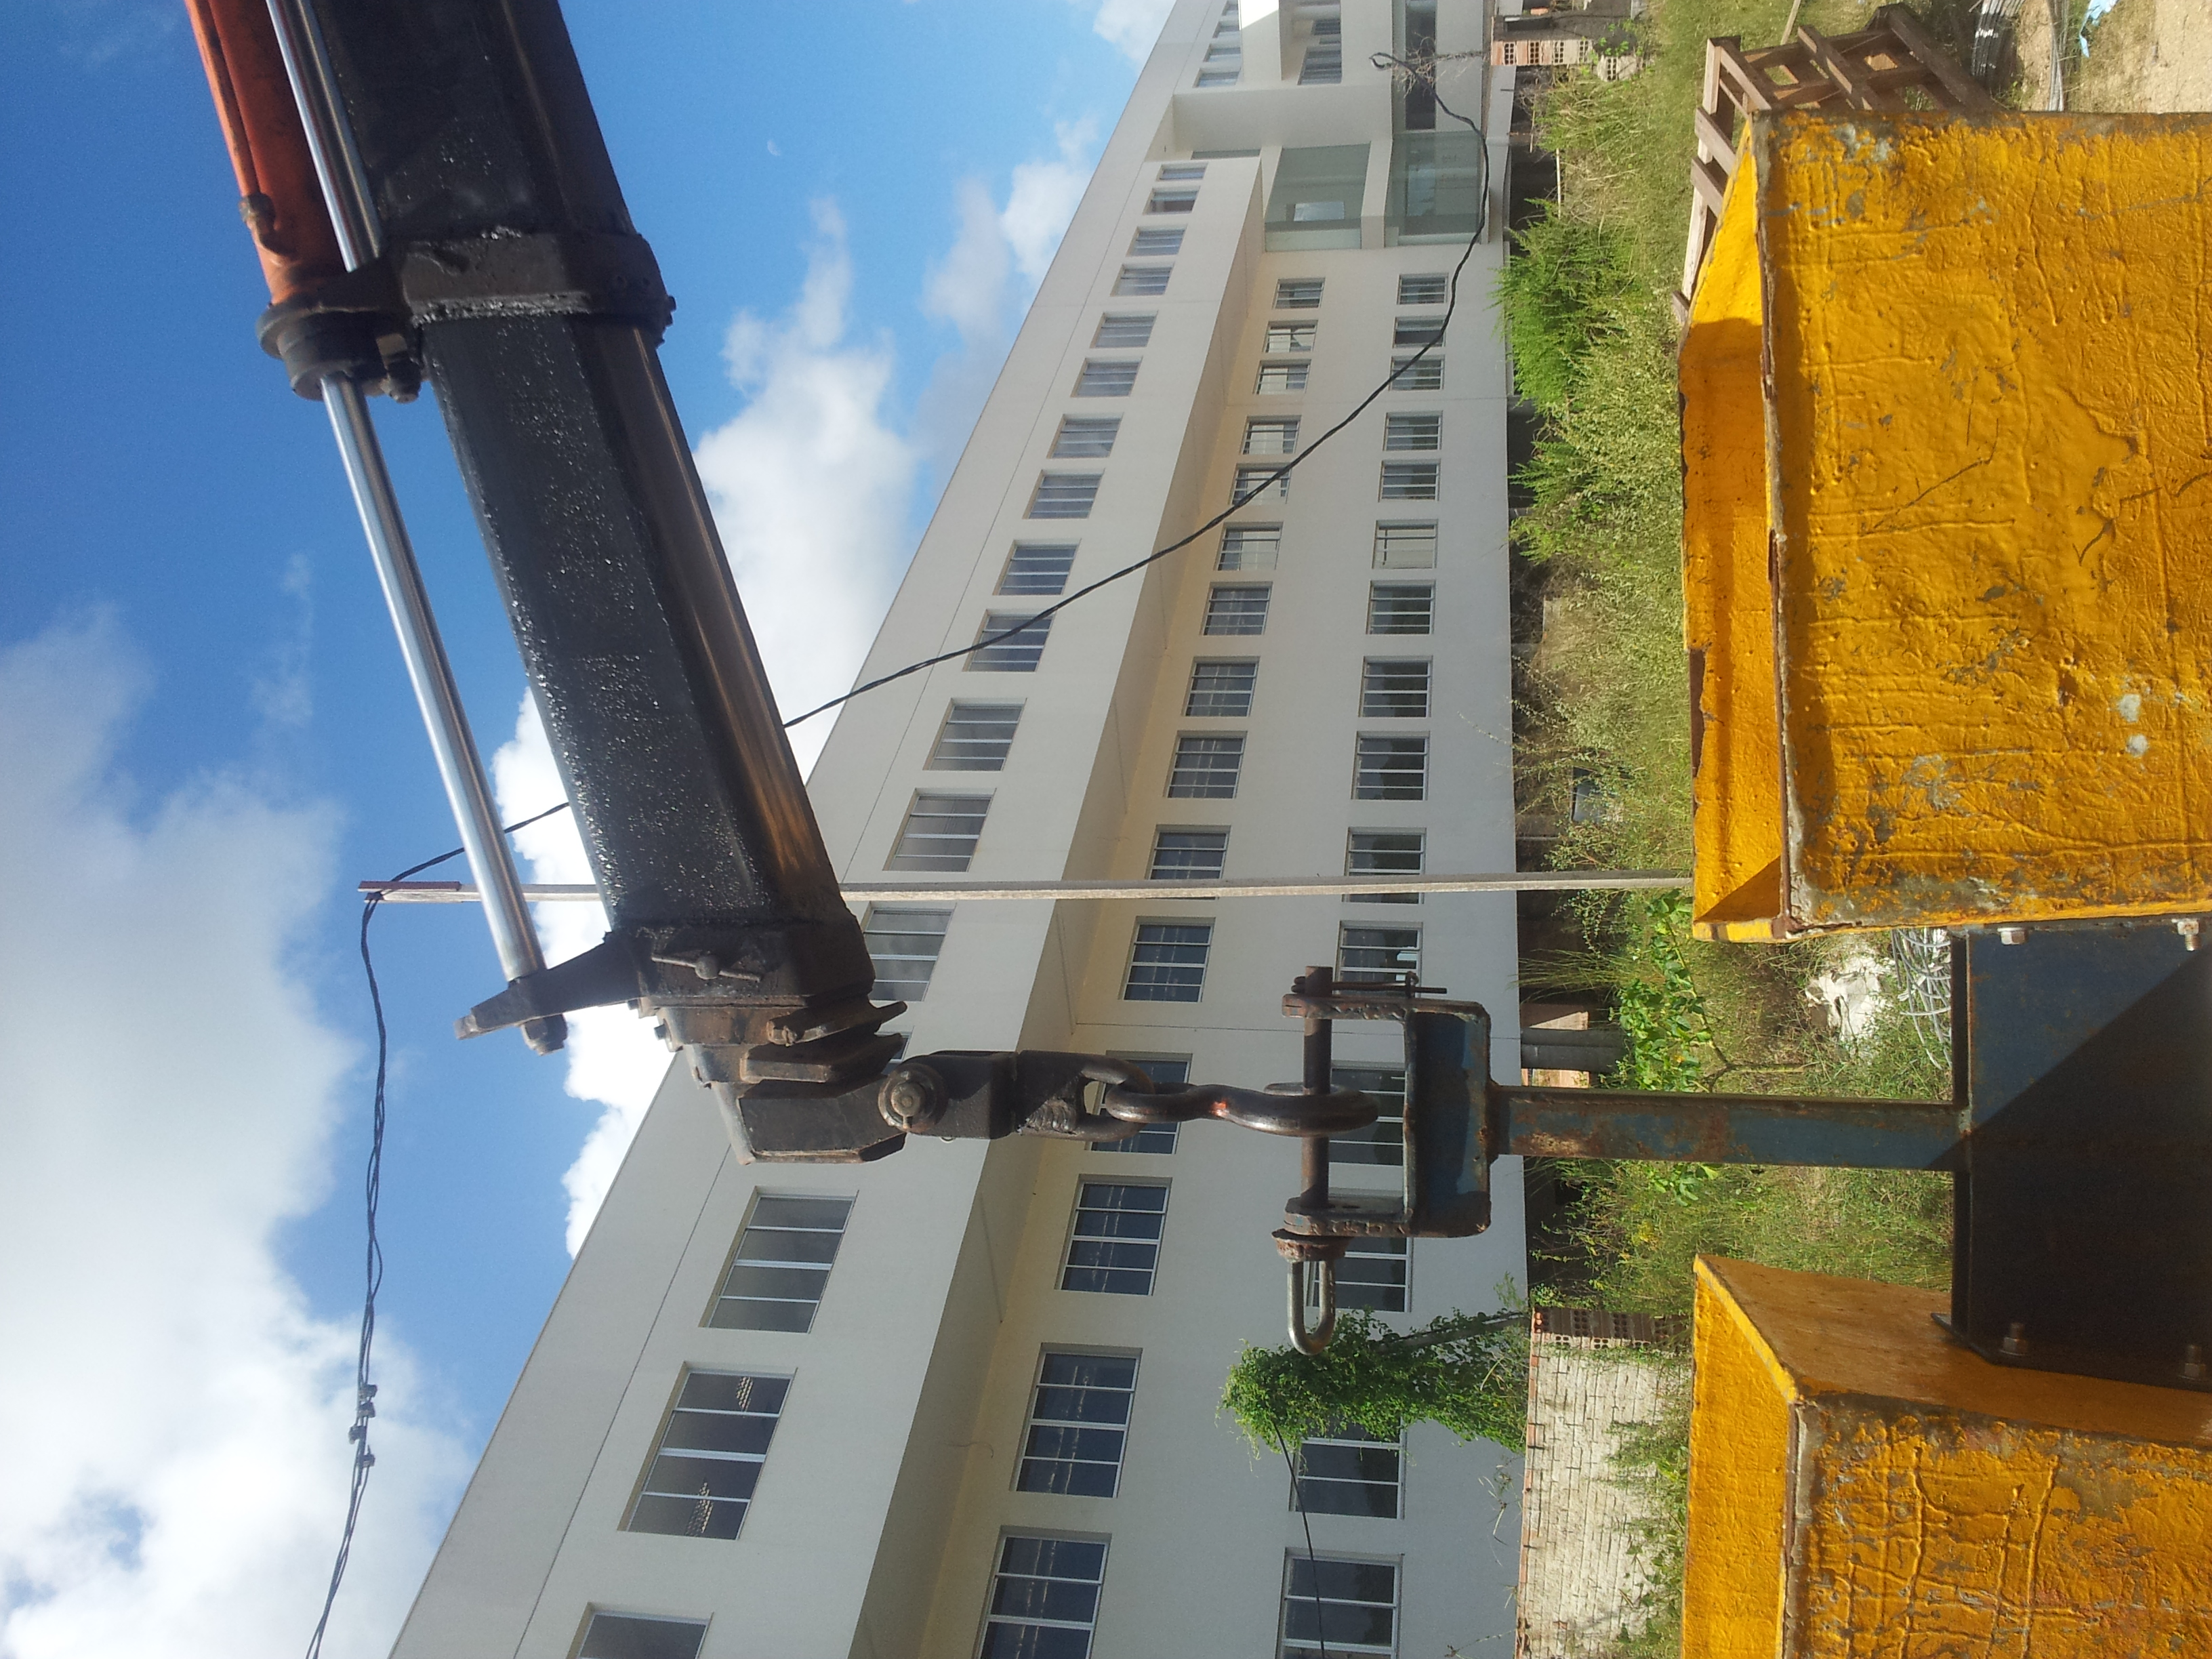
\includegraphics[width=4cm,height=4cm, angle = 270]{./pic/Muck2.jpg}}
\subfloat[Munck Extendido durante a montagem]{
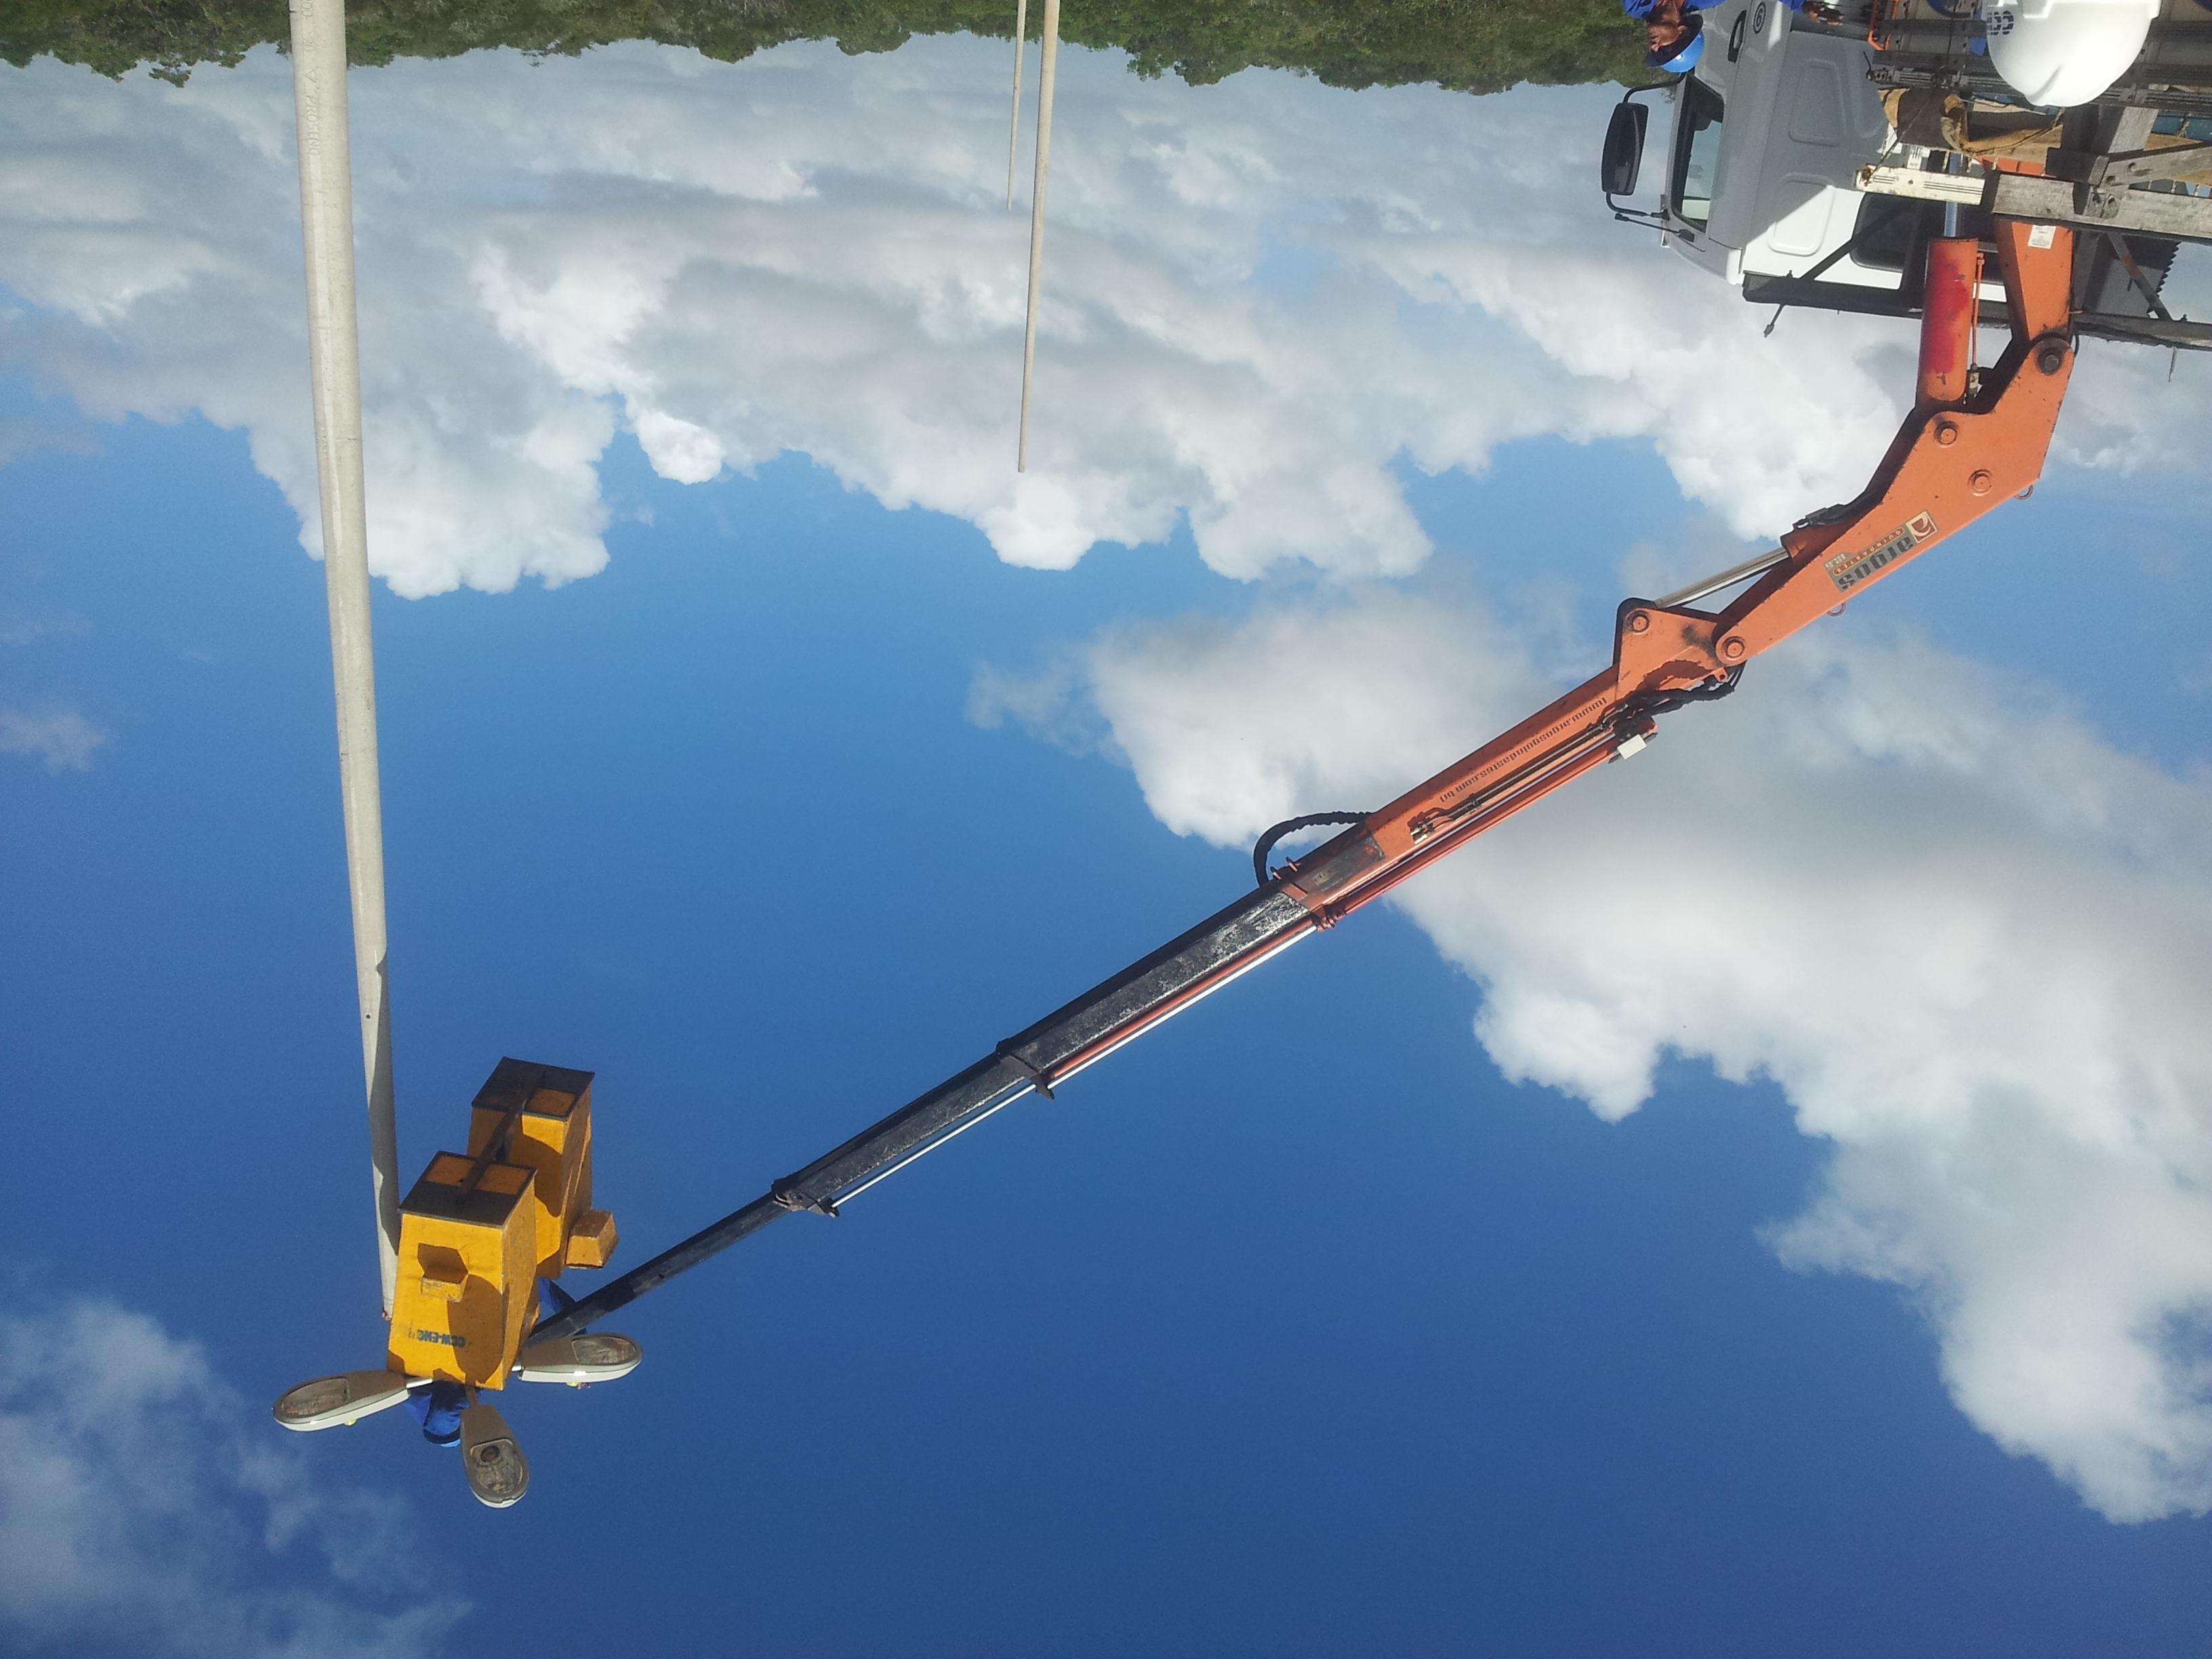
\includegraphics[width=4cm,height=4cm, angle = 180]{./pic/Muck_Extendido.jpg}}
\end{figure}


